%%%%%%%%%%%%%%%%%%%%%%%%%%%%%%%%%%%%%%%%%%%%%%%%%%%%%%%%%%%%%%%%%%%%%%%%%%%%
% AGUJournalTemplate.tex: this template file is for articles formatted with LaTeX
%
% This file includes commands and instructions
% given in the order necessary to produce a final output that will
% satisfy AGU requirements, including customized APA reference formatting.
%
% You may copy this file and give it your
% article name, and enter your text.
%
%
% Step 1: Set the \documentclass
%
%

%% To submit your paper:
\documentclass[draft]{agujournal2019}
\usepackage{url} %this package should fix any errors with URLs in refs.
\usepackage{lineno}
\usepackage[inline]{trackchanges} %for better track changes. finalnew option will compile document with changes incorporated.
\usepackage{soul}
\usepackage{natbib}
\usepackage{amsmath}

%-- new commands (QJ) --

\linenumbers
%%%%%%%
% As of 2018 we recommend use of the TrackChanges package to mark revisions.
% The trackchanges package adds five new LaTeX commands:
%
%  \note[editor]{The note}
%  \annote[editor]{Text to annotate}{The note}
%  \add[editor]{Text to add}
%  \remove[editor]{Text to remove}
%  \change[editor]{Text to remove}{Text to add}
%
% complete documentation is here: http://trackchanges.sourceforge.net/
%%%%%%%

\draftfalse

%% Enter journal name below.
%% Choose from this list of Journals:
%
% JGR: Atmospheres
% JGR: Biogeosciences
% JGR: Earth Surface
% JGR: Oceans
% JGR: Planets
% JGR: Solid Earth
% JGR: Space Physics
% Global Biogeochemical Cycles
% Geophysical Research Letters
% Paleoceanography and Paleoclimatology
% Radio Science
% Reviews of Geophysics
% Tectonics
% Space Weather
% Water Resources Research
% Geochemistry, Geophysics, Geosystems
% Journal of Advances in Modeling Earth Systems (JAMES)
% Earth's Future
% Earth and Space Science
% Geohealth
%
% ie, \journalname{Water Resources Research}

\journalname{Journal of Advances in Modeling Earth Systems (JAMES)}

\begin{document}

%% ------------------------------------------------------------------------ %%
%  Title
%
% (A title should be specific, informative, and brief. Use
% abbreviations only if they are defined in the abstract. Titles that
% start with general keywords then specific terms are optimized in
% searches)
%
%% ------------------------------------------------------------------------ %%

% Example: \title{This is a test title}

\title{Variability of the kinetic energy in seasonally ice-covered oceans.}

%% ------------------------------------------------------------------------ %%
%
%  AUTHORS AND AFFILIATIONS
%
%% ------------------------------------------------------------------------ %%

\authors{Josu\'e Mart\'inez-Moreno\affil{1,3}, Camille Lique\affil{1}, Claude Talandier\affil{1}, Quentin Jamet\affil{2}, Anne-Marie Treguier\affil{1}}

\affiliation{1}{Laboratoire d'Oc\'eanographie Physique et Spatiale (LOPS), University of Brest/IFREMER/IRD/CNRS, Brest, France}
\affiliation{2}{Service hydrographique et océanographique de la marine (SHOM), Brest, France}
\affiliation{3}{Now at the British Antarctic Survey, Cambridge, UK}


\correspondingauthor{Josu\'e Mart\'inez-Moreno}{josue.martinez.moreno@ifremer.fr}

\begin{keypoints}
\item Seasonal variations in Arctic sea ice significantly influence the ocean's scales of motion.
%The seasonality of the sea ice in the Arctic modifies the scales of motion of the ocean.
\item Between summer and winter, the dominant scales of motion in the Arctic transition from mesoscale to submesoscale. 
\item Sea ice dissipates preferentially the mesoscale range of motion in winter, and the inverse energy cascade enhances the mesoscale in summer.
\end{keypoints}

\begin{abstract}
  The seasonality of Arctic sea ice cover significantly influences heat, salt, buoyancy fluxes, ocean-ice stresses, and the potential and kinetic energy stored in the ocean mixed layer. This study examines the seasonal variability of oceanic scales of motion and cross-scale flux of kinetic energy in the seasonally ice-covered Arctic, using a high-resolution, idealized coupled ocean-sea ice model. Our simulations demonstrate pronounced seasonality in the scales of oceanic motion within the mixed layer, governed by distinct mechanisms during summer and winter. In summer, the inverse energy cascade transfers kinetic energy from the submesoscale towards the mesoscale range of motions. In winter, ice-induced dissipation suppresses kinetic energy and mesoscale motions, only allowing the persistence of submesoscale features. These results underscore the critical role of sea ice in modulating the seasonal dynamics of oceanic motion and their dominant scales, a behavior markedly different from that in the open ocean. Thus, understanding these coupled processes is essential for improving predictions of the ocean's energy evolution as the Arctic transitions toward a summer ice-free regime.
\end{abstract}

\section*{Plain Language Summary}

The seasonal changes in Arctic ice cover significantly influence heat, salt, and energy transfers within the ocean. This study employs a high spatial resolution model to investigate how these variations affect the seasonality of ocean currents and energy distribution throughout the year. Our findings reveal that the scale of ocean motion and the amount of kinetic energy differ between summer and winter. In summer, ocean scales exceed 5 km and exhibit higher energy levels. Conversely, in winter, sea ice dissipates oceanic energy, reducing energy levels, and limiting motion to scales smaller than 5 km. These results demonstrate that sea ice plays a pivotal role in shaping the seasonal dynamics of oceanic processes, a behavior that contrasts with the open ocean. Understanding these seasonal changes is critical for predicting how the Arctic will evolve as it transitions toward a summer ice-free state.


\section{Introduction}

Oceanic eddies are ubiquitous in the Arctic Ocean, particularly in seasonally ice-covered regions \citep{Cassianides_eddies_2023}. Arctic eddies are known to stir and mix ocean properties \citep{Fine_Microstructure_2018}, modulate the ocean stratification \citep{Pnyushkov_stratification_2018}, contribute to the equilibration of the large scale wind-driven circulation \citep{Lique_eddy_2015}, transport nutrients and tracers \citep{watanabe_nutrients_2014}, and transfer ocean heat vertically \citep{Bebieva_mixing_2016}. Eddies with horizontal length-scales of the same order as the first baroclinic Rossby deformation radius \citep[$\mathit{O}\sim 10\ km$ in the Arctic Basin;][]{Nurser_rossby_2014} are known in literature as mesoscale, while smaller scales are commonly referred to as submesoscale. Baroclinic instabilities in the ocean interior and within the mixed layer (ML), are known to convert potential energy to kinetic energy (KE) which results in the development of mesoscale and sub-mesoscale eddies \citep{FoxKemper_eddies_2008}.
Moreover, mesoscale and submesoscale eddies are able to transfer KE across scales from large scales toward smaller scales (the forward cascade) and from small to larger scales (the inverse energy cascade; \citealt{Srinivasan_submesoscale_2023, Naveira_KE_2022, Ferrari_KE_2009}). 
An improved understanding of the seasonality of KE and flow scales in the open ocean has been gained over the past decade \citep{Rocha_Seasonality_2016, Buckingham_submesoscale_2016, Qiu_seasonal_2014}. 
In a nutshell, in the open ocean, summer is marked by increased mesoscale KE and reduced energy within the submesoscale range due to an inverse energy cascade. In contrast, winter presents a slight decrease in mesoscale KE and a pronounced increase in submesoscale KE, driven by ML deepening and enhancement of ML instabilities, that fuels the inverse energy cascade in summer \citep{Yu_Seasonality_2023, Uchida_seasonal_2017,Sasaki_seasonal_2014}. 
In the ice-covered ocean, the seasonality of the ocean dynamics, stratification, and ML are strongly dominated by the growth, melt, and surface stress of the sea ice, thus we hypothesize that the seasonality of KE spectra could differ from the open ocean regime.

Several studies have explored the seasonal dynamics of submesoscale and mesoscale flows in polar regions, particularly under varying sea ice conditions. Using an idealized model configuration representing the multi-year sea ice pack, \citet{Mensa_seasonal_2017} showed that submesoscale KE increases during summer due to enhanced internal wave activity, whilst the mesoscale KE shows no seasonal variation, both in the ML and the ocean interior. 
In contrast, based on the analysis of realistic high-resolution simulations, \citet{Manucharyan_eddies_2022} and \citet{Liu_seasonal_2024} found some seasonal variability of the KE and the oceanic scales of motion (i.e. including both the mesoscale and submesoscale ranges of motion) in the seasonally ice-covered regions. In particular, \citet{Manucharyan_eddies_2022} noted a seasonal transition from an energetic mesoscale and weak submesoscale field in summer to a weak mesoscale and energetic submesoscale field in winter (see Fig. 3g in \citealt{Manucharyan_eddies_2022}), likely associated with the transition from high sea ice concentrations in winter to lower concentrations in summer. Additionally, they found that the vorticity variance was more strongly dissipated in winter than in summer due to the higher sea ice concentration. Although the findings of these studies might initially seem opposed, one need to remember that they consider different sea ice regimes: \citet{Mensa_seasonal_2017} focused on the ice pack, while the other two studies focused on the seasonal ice-covered zones and qualitatively described a dependency between the energetic ocean scales and the sea ice concentration. However, the seasonal transition of ocean scales and their energetics under sea ice, as the ocean shifts seasonally from ice-free to ice-covered conditions, remains to be fully characterized.

Determination from direct observations of the predominant ocean scales of motion seasonality in the Arctic is limited, but recent observational studies have provided some evidence supporting a seasonality of the mesoscale and submesoscale eddy fields. For instance, \citet{Meneghello_seasonal_2021} suggested using moorings and numerical simulations that the growth of surface mesoscale eddies in winter is modulated by sea ice friction, and \citet{Cassianides_eddies_2023} found hints of a seasonal variability within the mesoscale and submesoscale ranges in surface potential density spectra from Ice Tethered Profilers in the seasonally ice-covered Canadian and Eurasian basins. These seasonal variations of the potential density spatial variance are likely evidence of seasonal variations of the mesoscale and submesoscale fields under sea ice. Yet, it remains unclear which processes may be driving this seasonality. Here, we focus on the drivers of the energy variability at mesoscale and submesoscale, as well as the KE seasonality of these oceanic scales as the ocean transitions from ice-free to ice-covered conditions over a full seasonal cycle.

Sea ice dissipates ocean eddies through friction \citep{Ou_dissipation_1986}.  
Ice stress can act similarly to the `eddy-killing' process considered in ocean-atmosphere interactions \citep{Renault_eddy_killing_2016}, where wind stress dissipates the oceanic eddies. As sea ice drifts, it exerts stress on the ocean surface, and if the ice stress opposes the eddies' circulation, eddies will lose energy due to friction by the ice. In other words, the distribution of the stress experienced by the coherent eddies is asymmetrical in their azimuthal direction, thereby `killing' or weakening them, similar to how wind stress weakens eddies in ice-free regions. This interaction is the largest in seasonal ice-covered regions, where the mobility of the ice varies throughout the year. It is well known that `eddy killing' acts preferentially at given length-scales \citep{Rai_eddy_killing_2021}, thus we hypothesize that this ice-induced eddy dissipation may also act preferentially within a range of oceanic scales of motion and vary seasonally. This framework has been commonly used in ocean-atmosphere interactions, and here, we apply it to ocean-ice interactions.

This paper is structured as follows: Section \ref{Methods} details the methodology employed in our study. Section \ref{sec3.1} examines the seasonal transition of scales within the idealized simulation. In Section \ref{sec3.2}, we analyze the KE spectra, the generation of mesoscale and submesoscale eddies, and the seasonality of the forward and inverse energy cascade. Section \ref{sec3.3} explores the sources and sinks of KE of the simulation. Finally, Section \ref{conclusions} presents our discussion and conclusions, synthesizing the findings and their implications for the dynamics of the Arctic Ocean.

\section{Methods}
\label{Methods}

\subsection{Model configuration} \label{Model}

We use an hydrostatic ocean model (NEMO; \citealp*{NEMO_man}) coupled to an elasto-viscoplastic sea ice model (SI3; \citealp*{SI3_man}). The setup builds upon the idealized configuration presented in \citet{Martinez_eddies_ice_2025}, albeit at a higher horizontal resolution. It consists of a zonally reentrant channel that spans $300\ km$ meridionally, $200\ km$ zonally, and $500\ m$ in depth. The horizontal resolution is $250\ m$ and the vertical has 50 levels with variable spacing that increases from $2.5\ m$ at the surface to $19\ m$ at the bottom. This resolution was chosen to resolve mesoscale and submesoscale features arising from baroclinic instabilities prescribed in the initial conditions. The length-scales of these features are defined using the first baroclinic Rossby radius of deformation ($R_{D}$; \citealt{Chelton_geographical_1998}): 
\begin{linenomath*}
  \begin{equation}
    R_{D} = \frac{1}{f\pi} \int_{-h}^0 N dz,
    % \label{eq:eq8}
  \end{equation}
\end{linenomath*}
where $h$ is the model depth, $f$ is the Coriolis parameter (referenced at $80^\circ$N) and $N$, the Brunt-V\"ais\"al\"a frequency or the square root of the vertical stratification (Eq. \ref{eq:eq9}). Note that $N$ varies seasonally, thus the $R_D$ also presents a seasonal cycle. Following the approach by \citet{Callies_submesoscale_2013}, we distinguish between the mesoscale and submesoscale based on spatial scales: mesoscale refers to scales larger than the first deformation radius, while submesoscale refers to scales smaller than the first deformation radius. 

The main focus of the present study is the ML dynamics, thus a logarithmic bottom drag is implemented to control the flow length-scales generated by the halocline. Note that regardless of the choice of bottom drag, KE seasonality remains qualitatively consistent when using a free-slip bottom, though the flow intensity and scales are larger.
We use an f-plane approximation at $80^\circ\ N$ ($f=1.43\times 10^{-4} 1/s$), a velocity dependent bi-harmonic isopycnal tracer diffusivity, and a bi-harmonic horizontal viscosity. A nonlinear equation of state is used to compute density (EOS80; \citealt{EOS_80}). 
The vertical mixing is based on the turbulent kinetic energy closure from \citet{blanke_TKE_1993}. We use the Non-Penetrative Convective algorithm parameterization that mixes iteratively the water column until the density profile is stable. 
The atmospheric forcing consists of a daily climatology of shortwave radiation, longwave radiation, and air temperature built from ERA5 over the period 1979 to 2021 over the Arctic (north of $80^\circ\ N$; Fig. \ref{fig:fig_1}a). This forcing is spatially constant, and it does not include wind forcing. The seasonal cycle of the forcing allows the retreat and formation of sea ice during summer and winter, respectively. The surface fluxes between the ice-ocean-atmosphere are computed using the NCAR bulk formula \citep{Large_NCAR_2009}.

\begin{figure}
  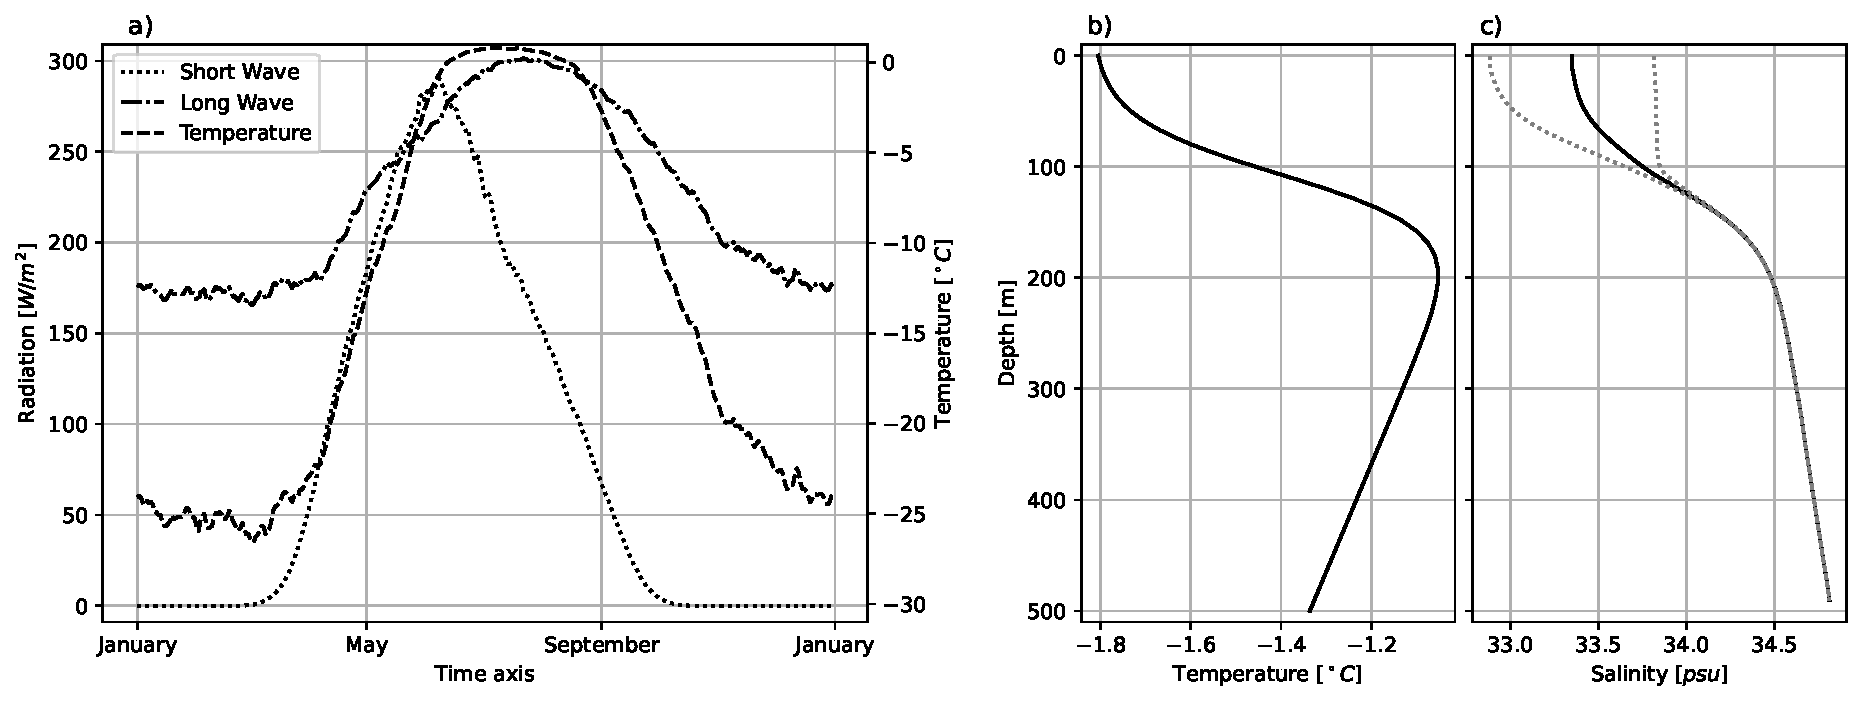
\includegraphics[width=1\textwidth]{Fig_1_forcing_and_profiles.pdf}
  \caption{Forcing and vertical initial profiles of the idealized configuration. (a) Incoming short wave radiation, incoming long wave radiation, and air temperature. Vertical profiles of (b) temperature and (c) salinity for the initial conditions of the simulation. In panel c, the dotted lines correspond to the northern and southern vertical salinity profiles of the simulation. Note that the temperature profile was adjusted to match the freezing point at the surface based on the mean salinity profile.}
  \label{fig:fig_1}
\end{figure}

The simulation is initialized with a meridional front prescribed only in the salinity field (Fig. \ref{fig:fig_2}a and b), since the density in the Arctic is mostly controlled by salinity. The front is generated by redistributing meridionally a $\sim 1\ psu$ salinity anomaly that extends down to $75\ m$ depth, with a fresh anomaly in the northern half of the domain (Fig. \ref{fig:fig_1}c). The temperature and salinity fields include noise in the top $75\ m$ to seed baroclinic instability. Our simulation is initialized from rest on May 1st with a sea ice thickness of 1 m over the entire model domain and it spins down over time. The background initial vertical temperature and salinity profiles resemble the observed vertical structure of the Arctic Canadian Basin with fresh and cold water masses above warmer and saltier waters below a $200\ m$ depth halocline (Fig. \ref{fig:fig_1}b and c; \citealt{Metzner_halocline_2023}). Baroclinic instabilities develop around the initial front and it takes a seasonal cycle for the ML, stratification, and sea ice to equilibrate. This seasonality of the simulation was found to be consistent across multiple horizontal resolutions: $2\ km$, $250\ m$, and $100\ m$. The analysis presented hereafter uses daily output during the second year of the $250\ m$ resolution simulation. The simulation reproduces the seasonality of the ice cover, with the sea ice extent maxima occurring in May (before the forcing maxima of incoming short wave radiation; Fig. \ref{fig:fig_1}a), and the domain is ice-free between August and October. 

\subsection{Energetics framework}

In this study, we are primarily interested in quantifying the contribution of spectral KE flux, vertical buoyancy fluxes and ice stress work in the seasonal variations of KE in our idealized simulation. Such contributions are part of the KE budget
\begin{linenomath*}
  \begin{align}
          \partial_t KE = - \nabla \cdot \left( \mathbf{u} KE \right)
          - \frac{1}{\rho_0}\nabla \cdot \left( \mathbf{u} p \right) + wb
          + \mathbf{u}_h \cdot \partial_z \left( \mathcal{A}_z \partial_z \mathbf{u}_h \right)
          - \epsilon,
  \label{eq:KEeqn_wb}
  \end{align}
\end{linenomath*}
obtained by vector multiplying the horizontal momentum equation of our hydrostatic primitive equation model by horizontal velocity $\mathbf{u}_h$, and using hydrostatic pressure and continuity equation for Boussinesq fluids to make explicit the contribution of vertical buoyancy fluxes $wb$. In equation  \ref{eq:KEeqn_wb}, 
$KE=\frac{1}{2}(\mathbf{u}_h \cdot \mathbf{u}_h)$ is the specific KE,
$\mathbf{u}=(\mathbf{u}_h,w)=(u,v,w)$ refers to the three-dimensional velocity field, $b=-g(\rho-\rho_0)/\rho_0$ is buoyancy, with $g$ the gravitational acceleration, $\rho_0$ the reference ocean density of $1026 kg/m^{3}$, and $\rho$ the potential density referenced to the sea surface.
$\mathcal{A}_z$ is the vertical viscosity coefficient computed by the vertical mixing scheme, and $\epsilon$ refers to dissipation.
The contribution of surface stress $\mathbf{\tau_o}$ (detailed in Section \ref{ice_stress}) enters the equation as the surface boundary condition of vertical dissipation of momentum, i.e. $\mathcal{A}_z\partial_z \mathbf{u_h}|_{z=\eta}=\frac{1}{\rho_0}\mathbf{\tau}_o$. 


For the first contribution we are interested in (spectral KE flux), we follow \citet{Capet_Mesoscale_2008} to form the equivalent of (Eq. \ref{eq:KEeqn_wb}) in Fourier space by vector multiplying the Fourier transform of the horizontal momentum equation by the complex conjugate of $\mathcal{F}(\mathbf{u}_h)$, with $\mathcal{F}$ the Fourier transform, retaining only the real part of the resulting equation. We adopt this strategy here, but only perform Fourier transform along the x direction in order to leverage from zonal homogeneity of our idealized setting, for which Fourier modes provide a suitable basis. 
For each zonal section, we thus obtain a KE budget in spectral space which can be synthesized as:


\begin{linenomath*}
\begin{equation}
  \frac{\partial}{\partial t}  \widehat{KE} (k_x,t) = T(k_x,t) + P(k_x,t) - D(k_x,t).
  \label{eq:eq5}
\end{equation}
\end{linenomath*}
Here, $\widehat{KE}=\Re \left[\mathcal{F}(\mathbf{u}_h)^* \cdot \mathcal{F}(\mathbf{u}_h) \right]$ is KE spectra, with $\Re$ representing the real part, $k_x$ is the wavenumber in the x direction, $P(k_x,t)$ is the forcing term including the conversion rate from potential energy to KE, $D(k_x,t)$  the dissipation including surface stress, and $T(k_x,t)$ emerges from the advection term of the momentum equation and corresponds to the transfer of KE among different spatial scales:

\begin{figure}[t]
  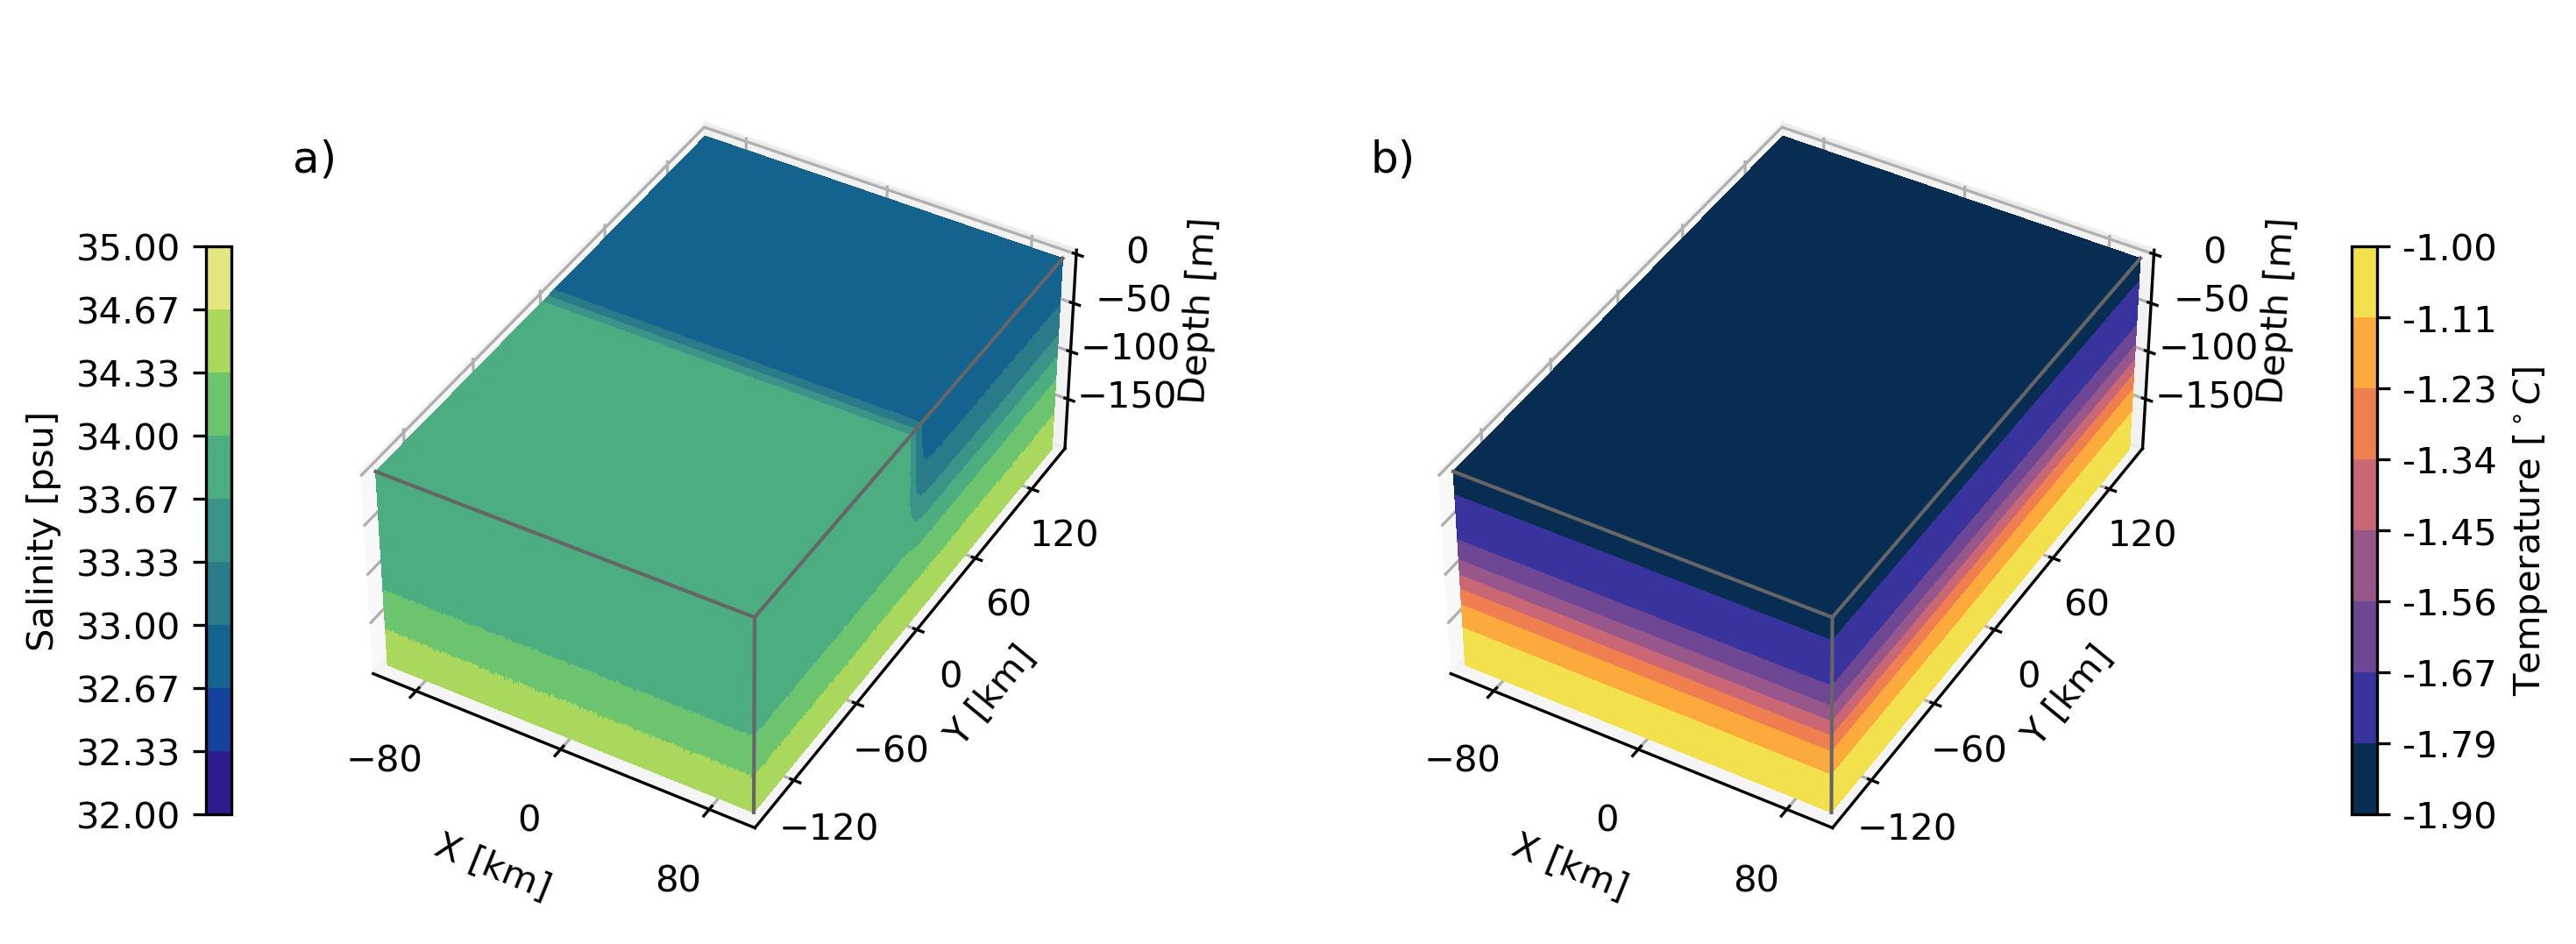
\includegraphics[width=1\textwidth]{Fig_2_init_conds.png}
  \caption{Initial conditions for the idealized coupled sea ice-ocean configuration. a) Initial ocean salinity with a fresher northern domain within the ML to develop baroclinic instabilities. The salinity difference between the northern and southern half of the domain is $1\ psu$. b) Initial ocean temperature representative of waters near the freezing point above a warmer subsurface layer.}
  \label{fig:fig_2}
\end{figure}

\begin{linenomath*}
\begin{equation}
  T(k_x,t) = \Re \left[ \mathcal{F}(u) ^* \mathcal{F}\left(u\frac{\partial u}{\partial x} + v\frac{\partial u}{\partial y} + w\frac{\partial u}{\partial z}\right) + \mathcal{F}(v) ^* \mathcal{F}\left(u\frac{\partial v}{\partial x} + v\frac{\partial v}{\partial y} + w\frac{\partial v }{\partial z}\right)  \right] / \Delta k_x.
  \label{eq:eq6}
\end{equation}
\end{linenomath*}
% where $\Re$ means the real part of the expression and $\mathcal{F}$ the Fourier Transform. 
The spectral KE flux $\Pi_Q$ is obtained by adding the 1D $T(k_x,t)$ from wavenumber $K'$ to the maximum available wavenumber ($k_x$; $\sim 4\ cpkm$),
\begin{linenomath*}
\begin{equation}
  \Pi_Q (K', t) = \sum_{k_x>K'}T(k_x,t). %\Delta k^2. 
  \label{eq:eq7}
\end{equation}
\end{linenomath*}

Based on the above definition, the KE spectra and KE flux were computed for 1D individual zonal transects (along the periodic size of the domain) and then averaged over the meridional direction, i.e. $\left<PSD(KE(x,t))\right>_y$ and $\left<\Pi_Q (K', t) \right>_y$, where $\left<\ \right>_y$ indicates the meridional average.

The spectral KE flux and KE spectra are computed between $-125\ km$ and $125\ km$ to avoid the effect of the northern and southern boundaries. The KE spectra is computed for snapshots on the 1st December, 1st March, 1st June, and 1st of September. The KE spectra spread corresponds to the median absolute deviation along the meridional direction. The spectral KE flux is averaged over each season and it represents the contribution of the mean transfer of energy from the start of one season to the start of the following one. For example, the summer energy flux corresponds to the mean energy transfer contributed to transition from the energy distribution on the 1st of June to that on the 1st of September. The spread of the KE flux was computed as the standard deviation in the meridional direction of the seasonally averaged KE flux. It thus represents the uncertainties in spectral flux associated with the meridional inhomogeneity of our configuration.

The second contribution of KE changes we are interested in is associated with kinetic to potential energy conversion encoded in $wb$.
It is common to Reynolds decompose this term to obtain statements of conversions between mean and eddy components of the (potential and kinetic) energy reservoirs. 
In our simulation, the geometry ensures that the average along the periodic direction (noted with a $\overline{\phantom{A}}$) represents the mean state of the domain and allows us to neglect the contribution of mean vertical velocities. Exchanges between mean potential and mean kinetic energy, i.e. $\overline{w}\overline{b}$, can thus be neglected, leanding to:
\begin{linenomath*}
\begin{equation}
  \overline{w'b'} \approx \overline{wb}.
  \label{eq:eq4}
\end{equation}
\end{linenomath*}

This term is commonly known as the baroclinic conversion rate, i.e. the conversion rate between eddy potential energy (EPE) and eddy kinetic energy (EKE), or eddy buoyancy flux \citep{Wunsch_vertical_2004}. Similarly, in the absence of zonal mean wind forcing, the zonally averaged mean flow is weak in amplitude as compared to the turbulent flow. In the results section, we primarily discuss the full KE estimates, as this mostly reflects the signature of turbulence.

\subsection{Instabilities}

Frontal structures within the ML can result in the generation of a submesoscale eddy field through ageostrophic and baroclinic instabilities \citep{FoxKemper_eddies_2008}. These instabilities extract potential energy by flattening isopycnals and inject KE into a ML eddy field. The generation of submesoscale eddies intensifies in regions with strong lateral buoyancy gradients, high vorticity, and weak vertical stratification, which can be quantified using the balanced Richardson number
\begin{linenomath*}
\begin{equation}
  Ri = \frac{N^2f^2}{M^4},
  \label{eq:eq8}
\end{equation}
\end{linenomath*}
where $N^2$, the vertical stratification, is defined as
\begin{linenomath*}
\begin{equation}
  N^2 = \frac{\partial b}{\partial z} %- \frac{g}{\rho_0}\frac{\partial \rho}{\partial z},
  \label{eq:eq9}
\end{equation}
\end{linenomath*}
$M^4$ is the square of the horizontal buoyancy gradient magnitude ($M^2=|\nabla_h b|$), i.e.,
\begin{linenomath*}
\begin{equation}
  M^4 = |\nabla_h b|^2 = \frac{\partial b}{\partial x}^2 + \frac{\partial b}{\partial y}^2.
  \label{eq:eq10}
\end{equation}
\end{linenomath*}

The contribution of the ML instabilities to the KE budget is quantified by the baroclinic conversion term (Eq. \ref{eq:eq4}; \citealt{Thomas_symmetric_2013}).
The characteristics of ML instabilities can be captured using the Eady theory \citep{Eady_eady_1949}, which was extended by \citet{Stone_baroclinic_1972} to include ageostrophic instabilities. The Eady time-scale is defined as:
\begin{linenomath*}
\begin{equation}
  T_s = \sqrt{\frac{54}{5}}\frac{\sqrt{1+Ri}}{|f|}.
  \label{eq:eq14}
\end{equation}
\end{linenomath*}
\citet{FoxKemper_eddies_2008} suggest that the Eady growth rate is a good estimate of the time-scale required to spin up of the instabilities. Thus, this linear theory is helpful in determining the likelihood of ML instabilities and ML eddies to be present in the simulations. 

By introducing the Richardson angle ($\phi_{Ri}$), the ML instability regimes can be classified into stable conditions and ageostrophic instabilities \citep{Thomas_symmetric_2013}:
\begin{linenomath*}
\begin{equation}
  \phi_{Ri} = tan^{-1}\left( -\frac{1}{Ri}\right).
  \label{eq:eq11}
\end{equation}
\end{linenomath*}
Ageostrophic instabilities could occur if the following criteria is met:
\begin{linenomath*}
\begin{equation}
  \phi_{Ri} < \phi_c  \equiv tan^{-1} \left(-\frac{\zeta_g}{f}\right),
  \label{eq:eq12}
\end{equation}
\end{linenomath*}
where $\zeta_g$ is the vertical component of the absolute vorticity of the geostrophic flow. Due to the hydrostatic approximation in NEMO, the ocean model can only represent ageostrophic instabilities with $N^2>0$, as any density inversion is mixed by the non-penetrative convection parameterization. Furthermore, the occurrence of baroclinic instability can be diagnosed in flows in which $Ri$ is $O(1)$ ($1 < Ri < 10$; \citealt{Haine_instability_1998}), since $Ri$ quantifies the magnitude of the slope of the buoyancy gradients (i.e. isopycnal tilting). 

\subsection{Eddy dissipation by sea ice}
\label{ice_stress}

The stress at the ocean surface ($\boldsymbol{\tau}_o $) is estimated by adding the quadratic form stress drag from the atmosphere and the ice as follows:
\begin{linenomath*}
\begin{equation}
  \boldsymbol{\tau}_o = (1 - A) \boldsymbol{\tau}_a +  A \boldsymbol{\tau}_i,
  \label{eq:eq15}
\end{equation}
\end{linenomath*}
where $A$ is the ice concentration, $\tau_a = \rho_a C_{Da} | \mathbf{u}_a - \mathbf{u}_o | \left(\mathbf{u}_a - \mathbf{u}_o\right)$ the atmosphere stress, $\rho_a$ the atmosphere density, $C_{Da}$ the air-ice drag coefficient, $\mathbf{u}_a$ the wind velocities at 10m, $\mathbf{u}_o$ the surface ocean velocities, and $\tau_i$ the ice stress. As the winds are set to zero in our simulation, we obtain:
\begin{linenomath*}
  \begin{equation}
    \boldsymbol{\tau}_o \approx A \boldsymbol{\tau}_i.
    \label{eq:eq16}
  \end{equation}
\end{linenomath*}
Note that setting up the wind velocities to zero, i.e. $u_a=0$, results in a positive stress (negative wind work), i.e. a small sink of energy everywhere in our domain particularly during the ice-free months when the ice concentration $A$ is small. 

The stress exerted by the sea ice into the ocean is equal to: 
\begin{linenomath*}
\begin{equation}
  \boldsymbol{\tau}_i = \rho_0 C_D | \mathbf{u}_i - \mathbf{u}_o | \left(\mathbf{u}_i - \mathbf{u}_o\right).
  \label{eq:eq17}
\end{equation}
\end{linenomath*}
Here, $C_D$ is the drag coefficient of $12\times10^{-3}$, chosen to be consistent with typical values used in high-resolution pan-Arctic simulations and within the observed range of drag coefficients in the Canadian Basin \citep{Cole_drag_2017, Dupont_creg_2015} and $\mathbf{u}_i$ the ice velocity. 
Analogous to the wind work and eddy killing proposed by \citet{Renault_coupling_2016}, we define the ice work or ice-induced eddy dissipation ($FK$) as:
\begin{linenomath*}
\begin{equation}
  FK = \frac{1}{\rho_0} \left( \overline{\tau_{i_x} u_i} + \overline{\tau_{i_y} v_i} \right)
  \label{eq:eq18}
\end{equation}
\end{linenomath*}
where $u_i$ and $v_i$ are the zonal and meridional ice velocities, $\tau_{i_x}$ and $\tau_{i_y}$ are the zonal and meridional surface ice stresses. This ice work can act to dissipate the energy contained by the eddy field, and using spectral analysis of the ice work, we can estimate the scales at which the eddy field is dissipated by the sea ice stress. Analogous to the KE energy spectra, we estimate the spatial scales in which ice work acts by computing the ice work spectra along the zonal direction of our idealized set up.

\section{Results}
\label{results}

\subsection{Seasonality of the ice-ocean conditions}
\label{sec3.1}

The seasonality of the atmospheric forcing (air temperature, incoming shortwave, and longwave radiation; Fig. \ref{fig:fig_1}a) are reflected in the seasonality of the domain averaged sea ice thickness, and temperature and salinity profiles (Fig. \ref{fig:fig_3}a and b). The sea ice thickness (overlaid to Fig. \ref{fig:fig_3}a) shows a characteristic seasonal cycle ranging from $0\ m$ in summer to $\sim 2\ m$ thickness in May. 
The ML, defined as the depth at which the difference in density exceeds the threshold value of $0.01\ kg/m^{3}$ with respect to a reference at $10\ m$ depth, has a significant seasonal variability from $\sim 11\ m$ in summer to $\sim 94\ m$ in winter (solid line in panels of Fig.\ref{fig:fig_3}). During summer, sea ice melt releases freshwater at the ice-ocean interface, forming a shallow summer ML. Additionally, a surface warm layer forms and becomes trapped below the ML, forming a remnant layer that persists until the next winter between the ML and the halocline. The trapped heat in this remnant layer is known to modulate the growth of sea ice in the following season as the ML deepens and warm water from this layer is entrained into the ML \citep{Cole_Remnant_2010,Mensa_seasonal_2017}. In winter, sea ice growth rejects brine and deepens the ML. Our simulations have a slightly deeper ML than the basin averaged winter ML depths observed in the Arctic ($\sim 60\ m$; \citealt{Zhai_seasonal_2023}). The ML temperature in winter remains near the freezing point (a function of salinity and pressure; \citealt{EOS_80}).
In May, at the start of the melting season, the ML initially shoals, then briefly deepens, before eventually stabilizing at a shallower depth. This occurs because the ocean surface freshens and the freezing point raises, allowing sea ice to briefly regrow, which causes brine rejection and a sudden deepening of the ML.
As surface warming continues in response to the atmospheric forcing, the ML equilibrates and reaches a depth of $\sim 10\ m$ in summer. 
The vertical stratification also presents a seasonal cycle consistent with observations (Fig. \ref{fig:fig_3}c; \citealt{Cole_stratification_2024}). During winter, the surface layer thickens due to brine rejection and mixing, which weakens the vertical stratification. In contrast, in summer, the input of warm and fresh water at the surface increases buoyancy and strengthens the vertical stratification between the surface and the ocean interior.

\begin{figure}
  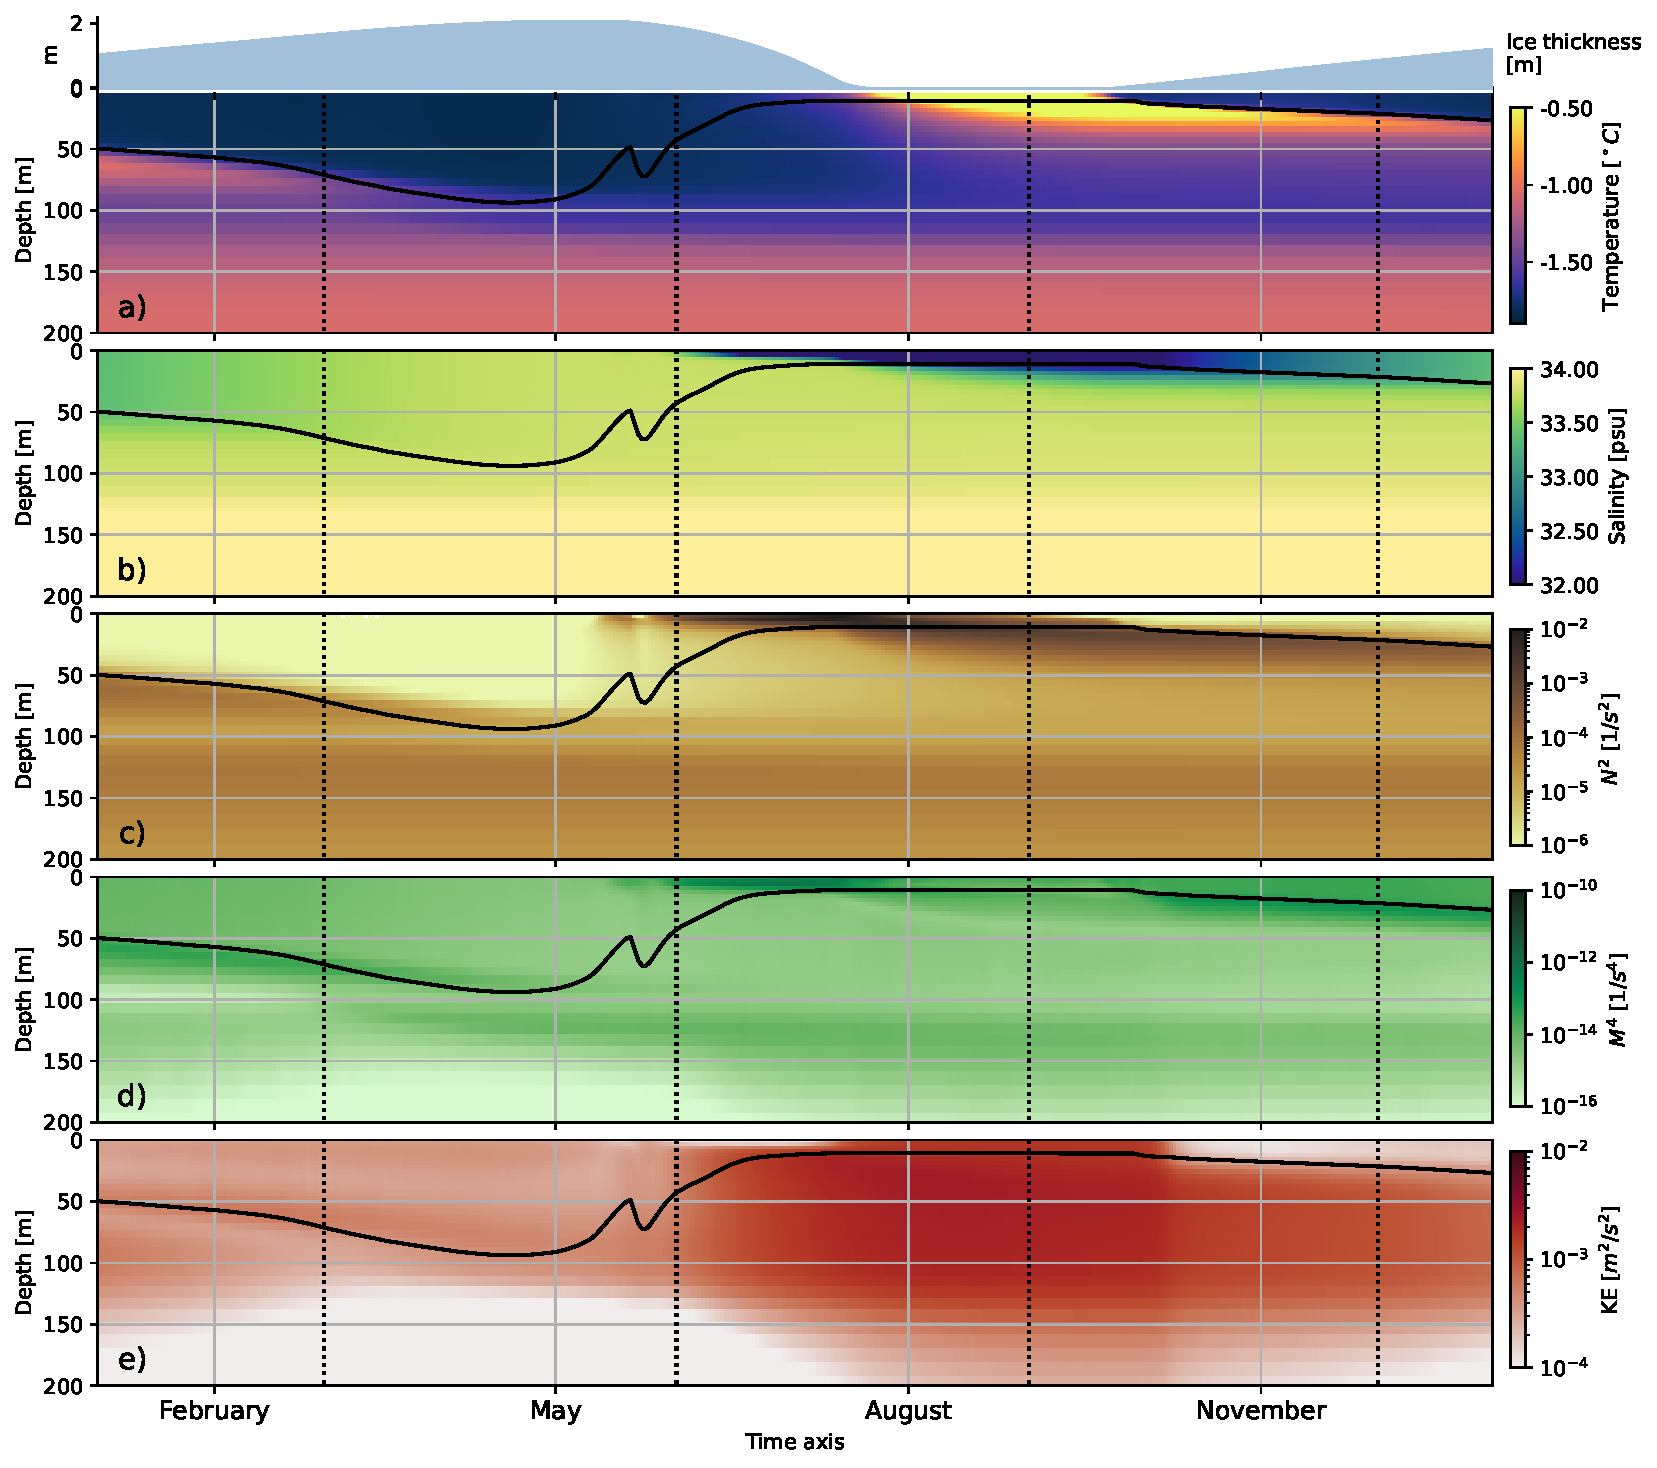
\includegraphics[width=1\textwidth]{Fig_3_hovemoller.pdf}
  \caption{Hovm\"oller diagrams during the second year of the simulation show the domain averaged (a) temperature, (b) salinity, (c) vertical stratification ($N^2$), (d) squared horizontal buoyancy gradients ($M^4$), and e) kinetic energy. Additionally, the mixed layer depth is shown with the black solid line in all panels. The ice thickness is shown above panel a). Vertical dotted lines correspond to the first day of the different seasons.}
  \label{fig:fig_3}
\end{figure}

The pattern seen in the vertical stratification is similar to that of the squared horizontal buoyancy gradients ($M^4$; Fig. \ref{fig:fig_3}d), albeit with a weaker value at the surface during the ice-free months (August-October). During the ice-covered period (winter and spring), the domain-averaged horizontal buoyancy gradients strengthen near the ML depth, likely linked to ML instabilities and the presence of submesoscale processes \citep{Timmermans_horizontal_2012}. In fact, $M^4$ is of the same order of magnitude as $N^2f^2$ (see Eq. \ref{eq:eq8}), therefore ML instabilities and submesoscale eddies are expected to be present in the simulation \citep{FoxKemper_eddies_2008}.
The time series of KE reveals a more energetic ocean in summer, starting when the ice starts to melt (June) and ending when ice re-growths in October (Fig. \ref{fig:fig_3}e). During the same period, the surface layer associated with high KE thickens from $\sim 100\ m$ depth to up to $\sim 150\ m$ depth. These summer changes are likely consequence of the absence of sea ice, which reduces dissipation of ocean currents and facilitates the generation of eddies in the halocline \citep{Zhao_eddy_2014}. During the rest of the year, KE is at least one order of magnitude smaller and large values are generally constrained to the top $\sim 100\ m$ depth. The Hovm\"oller diagram seasonality is not entirely periodic, despite this, the modeled seasonal cycle remains consistent during the subsequent years of the simulation (not shown).

\begin{figure}[t!]
  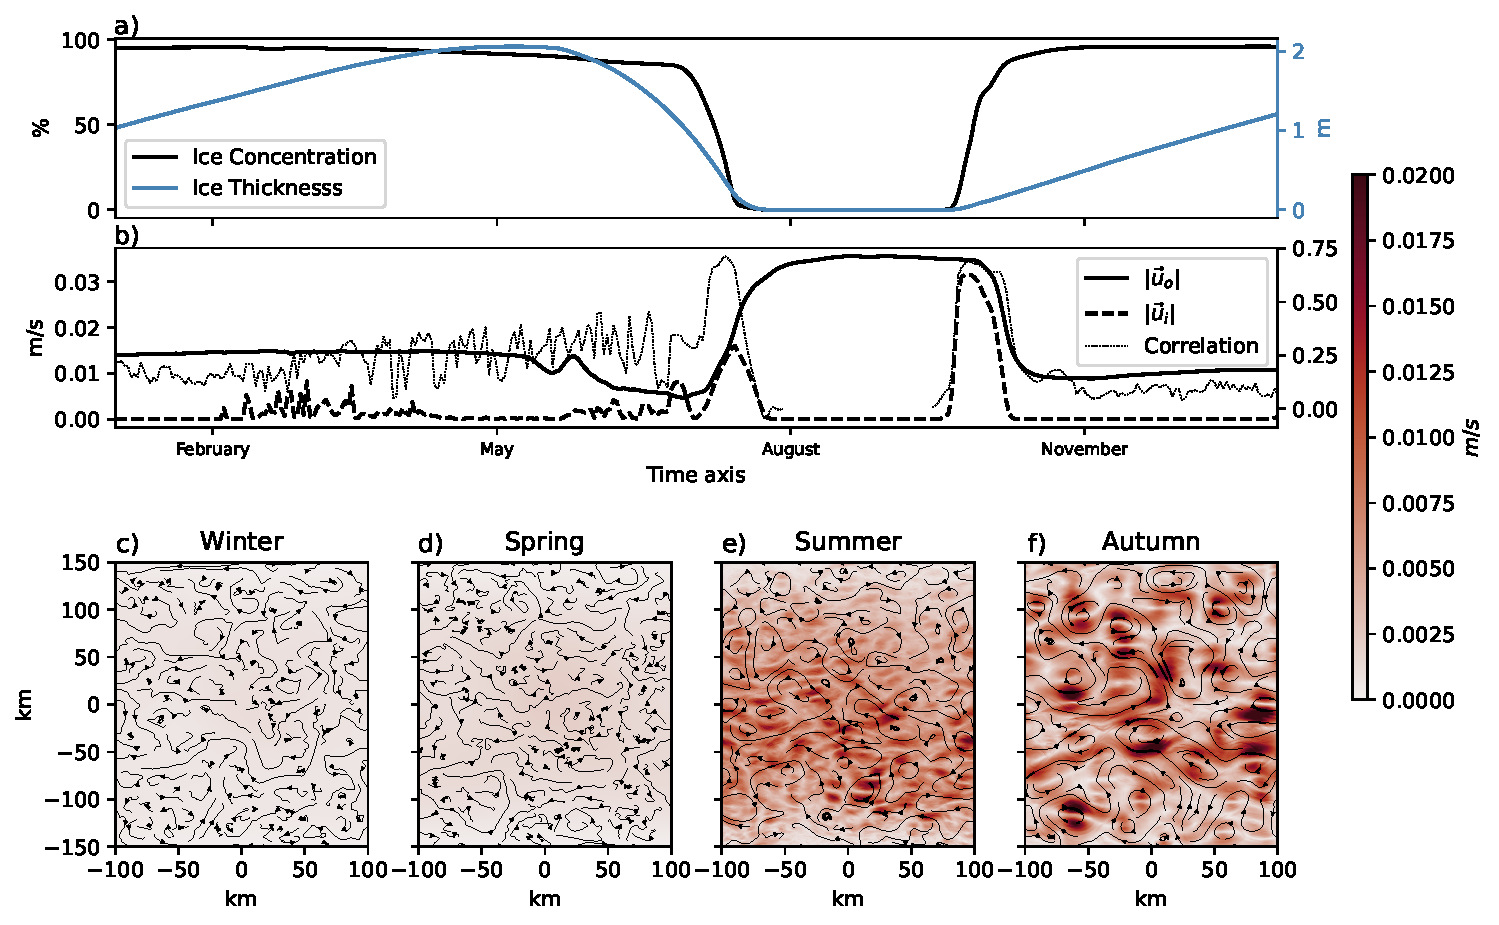
\includegraphics[width=1\textwidth]{Fig_4_ice_scales.pdf}
  \caption{Time-series of the domain average (a) ice concentration and thickness, and (b) ocean surface velocity magnitude ($|\vec{u}_o|$) and ice velocity magnitude ($|\vec{u}_i|$). The dotted line corresponds to the Spearman correlation coefficient between the ocean and ice velocities for each day of the second year of the simulation. Seasonally averaged ice velocity magnitude and ocean velocities streamlines in the presence of sea ice (i.e. where ice concentrations are larger than 0\%) are shown for c) winter, d) spring, e) summer, and f) autumn.}
  \label{fig:fig_4}
\end{figure}

The seasonality of KE is further explored by comparing time series of the ocean velocity magnitude ($|\vec{u}_o|$) and ice velocity magnitude ($|\vec{u}_i|$; Fig. \ref{fig:fig_4}b). The time series of the surface ocean velocities show three distinct periods; i) a relative constant average ocean velocity as the ice thickness increases in response to the atmospheric forcing, ii) a decrease in June-July due to the thin, fresh, and shallow ML at the beginning of the melting season that decouples the ocean velocities near the surface from those in the interior (see Fig.\ref{fig:fig_3}), and iii) a period characterized by strong velocities once the ocean is ice-free.
On average, the ocean velocity is approximately $0.02\ m/s$, and it peaks during the ice-free months (Fig. \ref{fig:fig_4}a). The ice velocity is on average $\sim 0.003\ m/s$ and it exhibits two prominent peaks: one in July, during ice melt, and another in October, during ice refreezing (Fig. \ref{fig:fig_4}b). During these two periods and because our simulations exclude wind forcing, the velocities of ice and ocean are highly correlated, with a correlation coefficient of $\sim 0.7$ (Fig. \ref{fig:fig_4}b), indicating that the ice is moving at the same speed and scales as the ocean (free drift), thus resulting in minimal stresses between the ice and the ocean (Eq. \ref{eq:eq17}). In contrast, during winter and spring, the ice-ocean velocity correlation weakens, leading to increased stress as the motion of ice and ocean differ. Further evidence of this is shown in the seasonally averaged sea-ice velocity magnitudes and ocean currents in the presence of sea ice (Fig. \ref{fig:fig_4}c-f). In winter and spring (Fig. \ref{fig:fig_4}c and d), the ice velocity magnitude is nearly uniform, with a large-scale but very small speed across the simulation domain and the ocean currents are weak and their spatial pattern shows small scale motions. Conversely, in summer and autumn (Fig. \ref{fig:fig_4}e and f), the ice velocity patterns show greater variability and the ice velocity scales match the ocean's $R_D$ and ocean velocity scales. Note that there is an important change in the scales of motion observed in the ocean and sea ice velocities between spring (high ice concentrations) and autumn (low ice concentrations). This transition from ice-covered to ice-free conditions and vice-versa results in a seasonal variability of the ocean and ice velocities, which in turn modulate the ocean surface stress and the KE budget.

\begin{figure}[t!]
  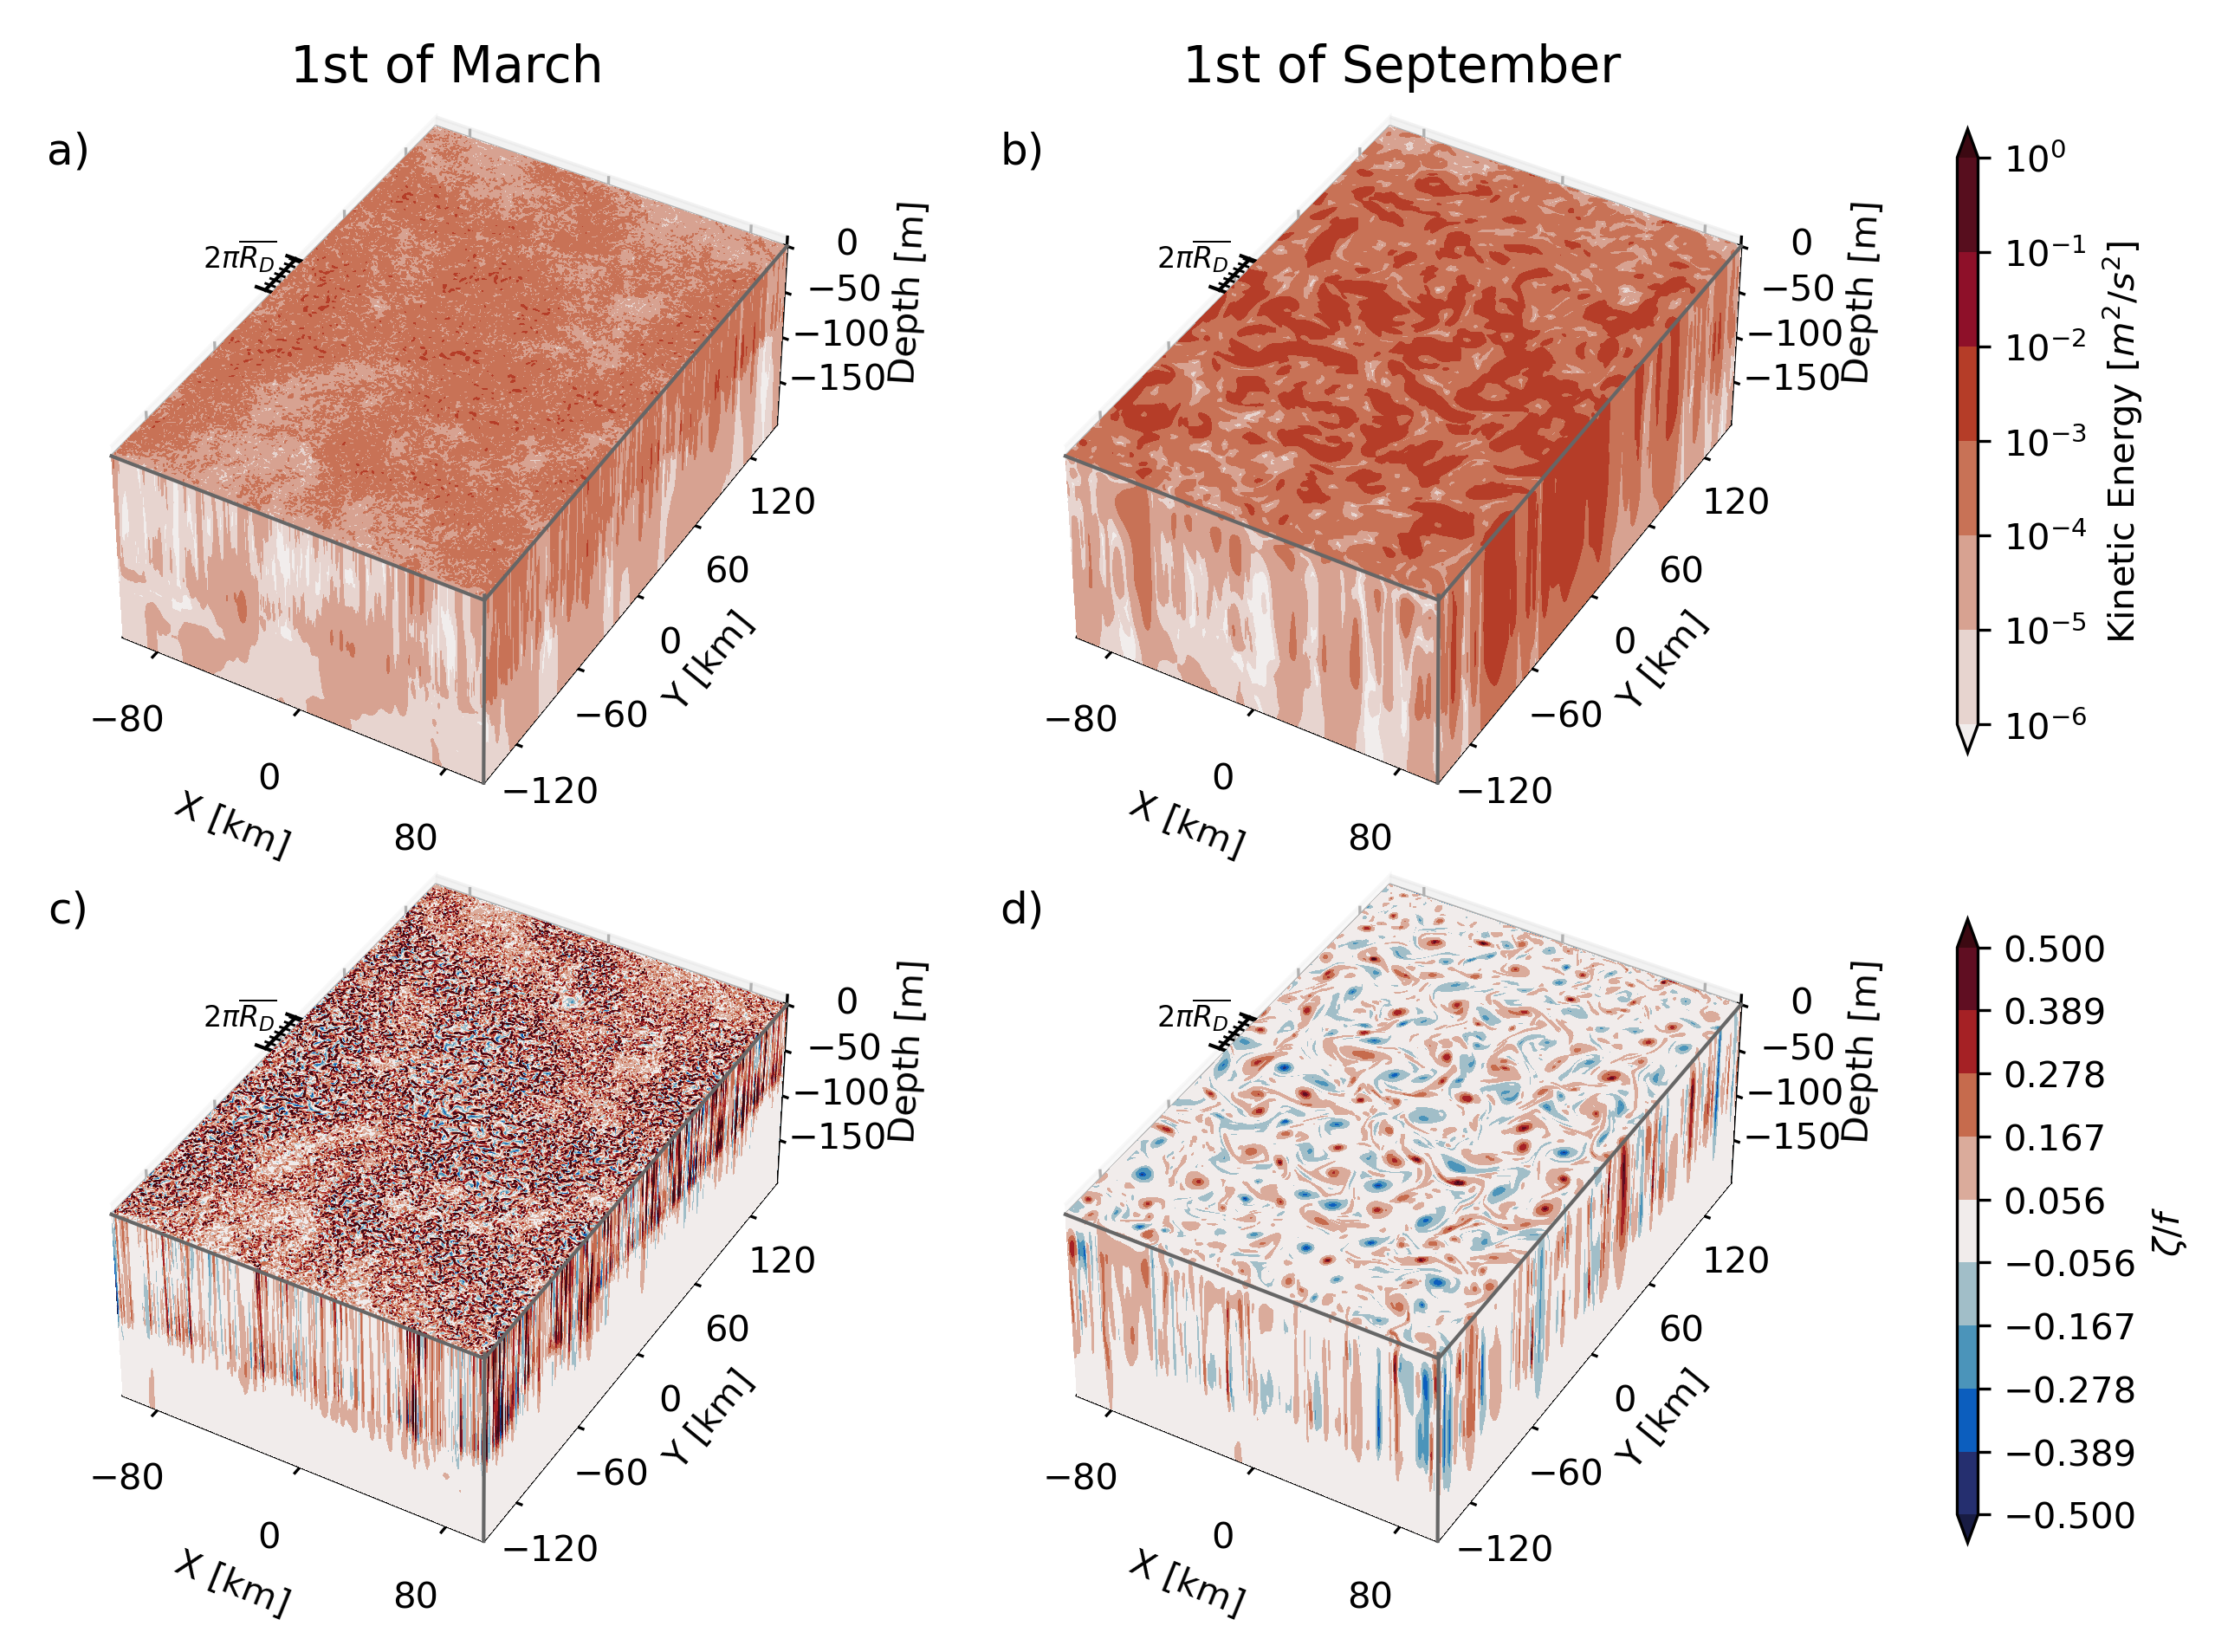
\includegraphics[width=1\textwidth]{Fig_5_KE_rossby.png}
  \caption{Snapshot on KE (top; panels a and  b) and normalized vorticity ($\zeta/f$) (bottom; panels c and d) on the 1st of March (left column) and the 1st of September (right column). The time mean Rossby radius wavelength is shown in all panels ($\lambda_r = 2\pi \overline{R_D}$).}
  \label{fig:fig_5}
\end{figure}

Figure \ref{fig:fig_5} shows summer and winter snapshots of the KE and normalized vorticity. In the winter snapshot (1st of March, Fig. \ref{fig:fig_5}a and c), the field is highly heterogeneous with scales smaller than the winter first baroclinic Rossby radius of deformation ($R_{D} \sim 4.1\ km$). This spatial scale in addition to a mean KE over the first $100\ m$ of $\sim 1.6\times10^{-4}\ m^2/s^{2}$ and the large normalized vorticity values ($\zeta/f > 0.5$ ; Fig. \ref{fig:fig_5}c) suggest the presence of submesoscale dynamics during winter. In contrast, in summer (1st of September, Fig. \ref{fig:fig_5}b and d) the domain is ice-free and the scale of the flow become larger than the summer $R_D\sim 5.3\ km$, up to the wavelength $\lambda_r = 2\pi R_D \approx 33\ km$. The mean KE over the first $100\ m$ is $\sim 1\times10^{-3}\ m^2/s^{2}$, one order of magnitude larger than the KE in the winter snapshot, consistent with Figure \ref{fig:fig_3}b. This larger spatial scale in addition to an increase in KE and smaller normalized vorticity values ($\zeta/f < 0.5$; Fig. \ref{fig:fig_5}d) suggests the presence of mesoscale dynamics in summer. Overall, the deformation radius and the seasonal variability of the normalized vorticity corroborate the seasonality of the dominant flow scales from submesoscale in winter to mesoscale in summer. The subsequent sections elaborate on the potential drivers of KE seasonality, including the transfer of KE among the different spatial scales ($T(k_x,t)$), the conversion of EPE to EKE ($w'b'$), and the dissipation by sea ice. %We have chosen not to include the pressure work and vertical dissipation terms in our study, leaving them for future consideration elsewhere.

\subsection{Seasonality of the kinetic energy cascade}
\label{sec3.2}  

The KE spectra and spectral KE flux are calculated to quantify the scale seasonality and energy transfers between submesoscale and mesoscale. These length-scales are defined using the first baroclinic radius of deformation that presents a temporal variability (Fig. \ref{fig:fig_6}a). Hereafter, we use the time-mean $R_D$ ($\overline{R_D} \sim 4.5\ km$) to indicate the transition between scales belonging to the mesoscale ($>\overline{R_D}$) and submesoscale ($<\overline{R_D}$). 

The KE spectra for a snapshot at the beginning of each season are shown in Figure \ref{fig:fig_7}. Near the surface, at $5\ m$ depth (Fig. \ref{fig:fig_7}a), the KE spectra reveals a pronounced variability of the KE contained within each length-scale, particularly within the mesoscale range. This variability is exemplified by contrasting the spectra in ice free conditions (1st of September) and ice covered conditions (1st of March). 
During ice free months, the KE spectra exhibits more energy within the mesoscale range. This suggests a prevalence of eddies with a Rossby radius greater than the $\overline{R_{D}}$. In contrast, the spectra for the ice covered conditions reveal a decrease in the energy at mesoscale and a gain of energy at submesoscale, indicative of an intensified smaller-scale field ($<\overline{R_{D}}$). The 1st of December and 1st of June spectra resemble that of the 1st of March, because at these dates, the domain is fully ice-covered. Looking at the periods in which ice melts and forms, the spectra transitions between these two states. Evidence of this is shown in the monthly averaged spectra in Figure \ref{fig:fig_6}. These variations are consistent with the seasonality of KE in high-resolution realistic simulations (see Fig. 3g of \citealt{Manucharyan_eddies_2022}). At $150\ m$ depth, where the ocean environment is less influenced by surface fluxes and the ice cover (Fig. \ref{fig:fig_3}b), the KE spectra is less energetic. At this depth, a clear distinction emerges: September 1st and December 1st exhibit more energy across most of the KE spectra, whereas March 1st and June 1st show weaker energy levels. This difference is likely due to halocline eddy activity and the persistence of eddies in the remnant layer during autumn and winter.

%Furthermore, at this depth there is a difference between the 1st of September and 1st of December, and the 1st of March and 1st of June likely due to the generation of eddies within the halocline and reminiscent effect of eddies trapped in the remnant layer. %Despite this, Figure \ref{fig:fig_3}e shows a noticeable drop on the KE magnitude below $150m$ depth. 

\begin{figure}[h]
  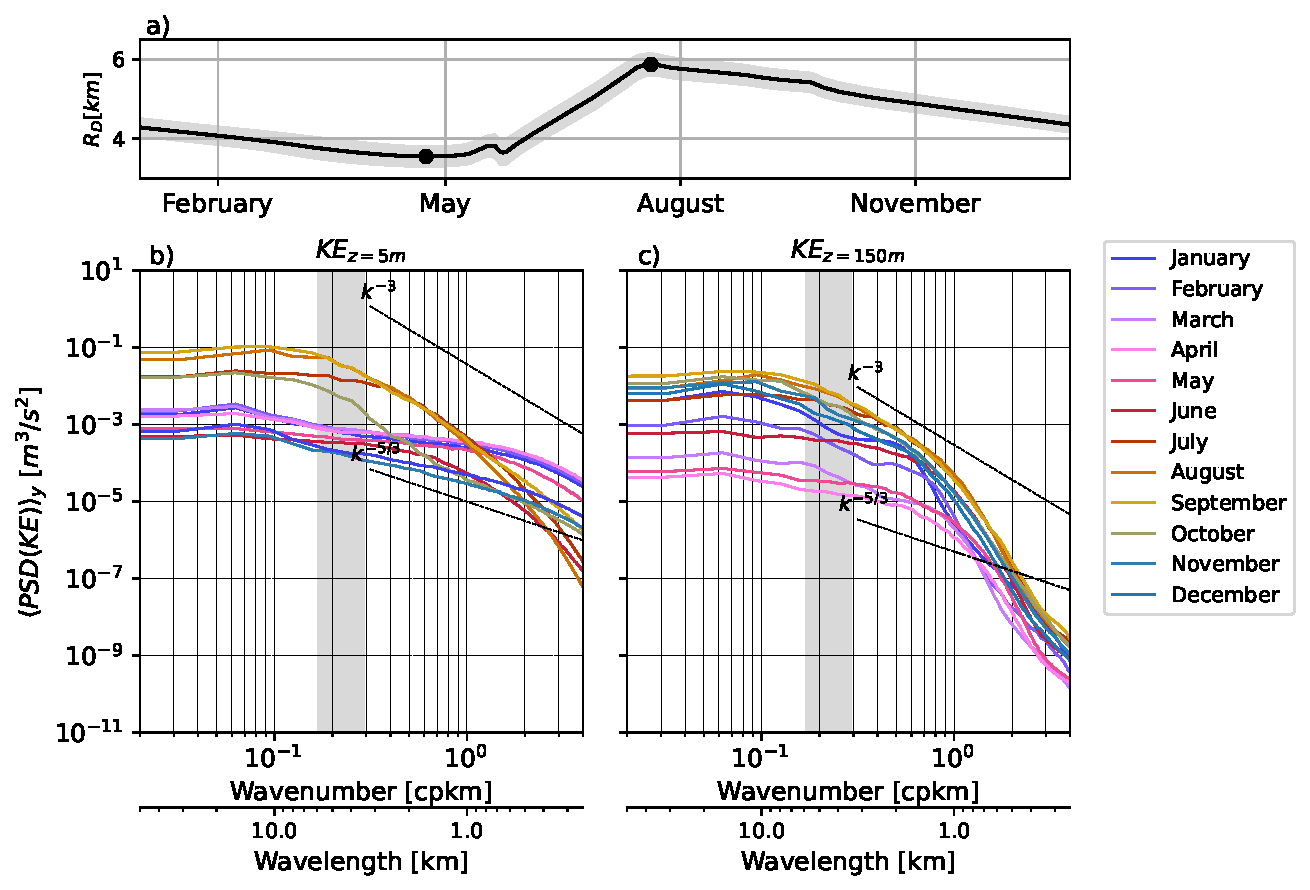
\includegraphics[width=1\textwidth]{Fig_6_spectra_2d_monthly.pdf}
  \caption{a) Time series of the domain average Rossby radius ($R_D$) for the second year of the simulation. The shading area correspond to the Rossby radius standard deviation, and the dots correspond to the $R_D$ maxima and minima of the year ($5.9\ km$  and $3.4\ km$, respectively).
  Monthly averaged kinetic energy spectra at b) $5\ m$ and c) $150\ m$ depth. Vertical shaded area in panels b) and c) matches the maxima and minima of the $R_D$ shown in panel a).}
  \label{fig:fig_6}
\end{figure}


\begin{figure}[t!]
  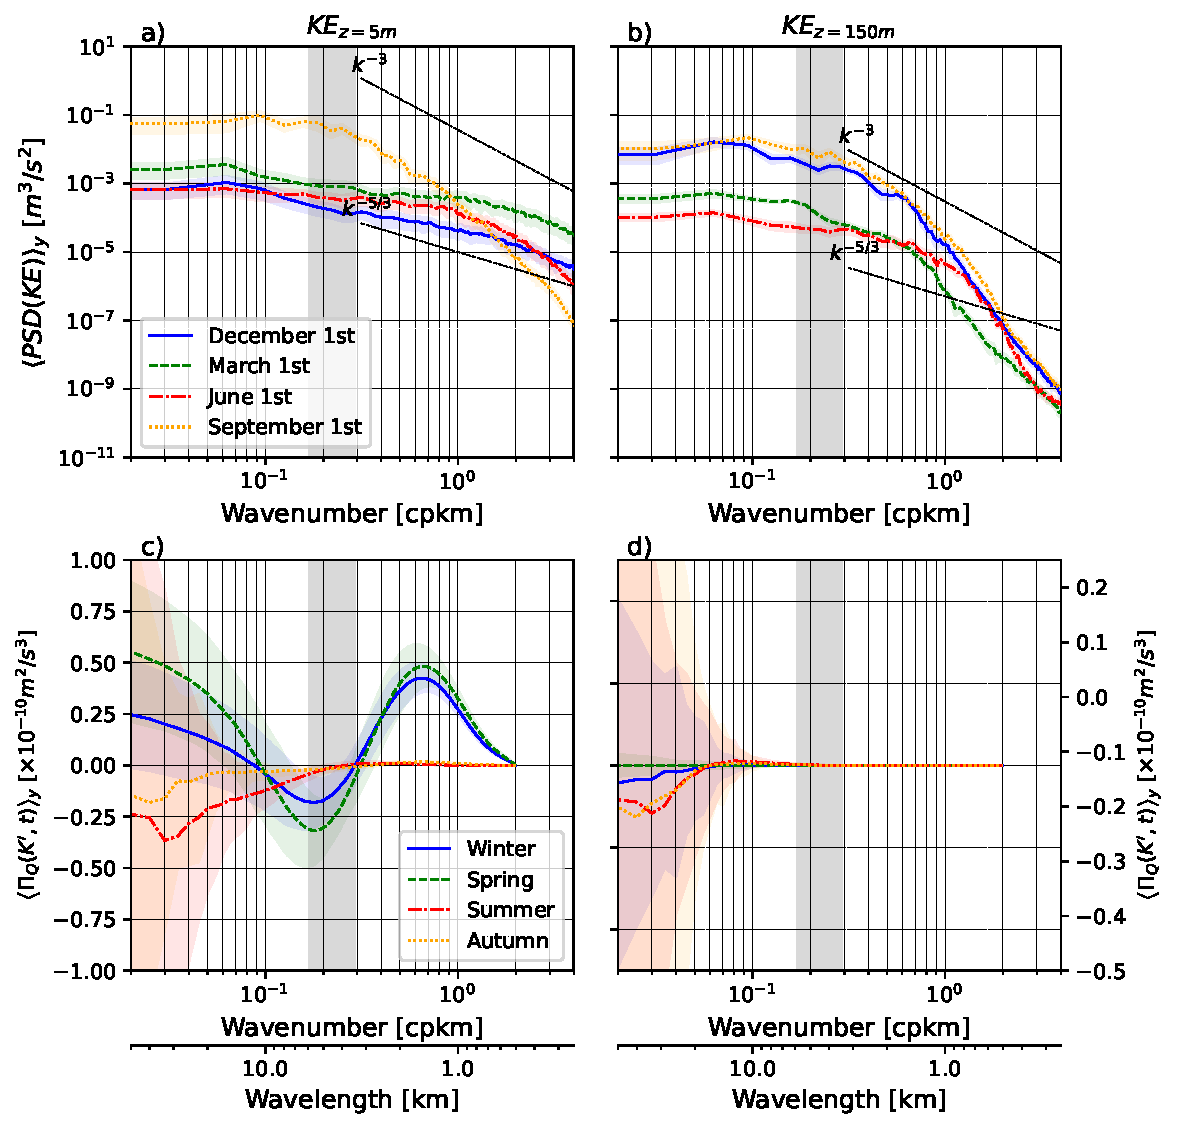
\includegraphics[width=1\textwidth]{Fig_7_spectra_and_flux_first_snapshots.pdf}
  \caption{KE spectra snapshots a) at $5\ m$ depth and b) at $150\ m$ depth for the first day of each season (1st December, 1st March, 1st June, and 1st of September). KE flux averaged for each season at c) $5\ m$ and d) $150\ m$ depth. The dashed lines correspond to the $-3$ and $-5/3$ slopes typical of KE spectra. The grey vertical shaded area correspond to the Rossby radius ($R_D$) range within the second year of the simulation (see Fig. \ref{fig:fig_6}a). In panels a) and b) the shaded areas correspond to the median absolute deviation in the meridional direction of the KE spectra, and in panels c) and d) the shaded areas correspond to the standard deviation in the meridional direction for the seasonally averaged KE flux.}
  \label{fig:fig_7}
\end{figure}

% Spectra slopes are a well known diagnostic diagnostic of ocean turbulence.
According to 2D turbulence \citep{Charney_turbulence_1971,Vallis_atmospheric_2017}, the open-ocean power laws (KE spectral slopes) associated with energy cascades are approximately $k^{-3}$ and $k^{-5/3}$ (i.e. forward cascade and inverse energy cascade respectively), where $k$ is the wavenumber. The recent study by \citet{Manucharyan_eddies_2022} on ice-covered regions suggests that these slopes may differ from the conventional values observed in the open ocean. Similarly, our simulation's spectral slopes differ from those derived from 2D turbulence theory, likely due to the contribution of the vertical component of the flow within the ML \citep{Schubert_cascade_2020}. Despite this, within the ML, spectral slopes $\sim k^{-5/3}$ can be attributed to an inverse energy cascade. They are prominent in our simulations on the ice-covered dates of December 1st, March 1st and June 1st for most of the wavenumbers, including the mesoscale and submesoscale ranges. In September 1st, these slopes are only observed within the mesoscale range of motion. Slopes $\sim k^{-3}$, associated with the direct enstrophy cascade in the open ocean, are only evident in September 1st for scales smaller than the $\overline{R_D}$, i.e. over the submesoscale range.

Power laws are a good indication of the forward cascade and inverse energy cascades \citep{Vallis_atmospheric_2017}, but a more quantitative estimate of the seasonal variability of the cascades is performed by computing the KE fluxes (Eq. \ref{eq:eq7}). The seasonally averaged spectral fluxes correspond to the energy transfer contributing to the transition from the energy distribution from the snapshot of the spectra at the beginning of a given season to the snapshot of the spectra at the beginning of the following season. Positive values of the KE flux indicate a forward KE energy cascade (KE energy is transferred from large to small scales), while negative values correspond to the inverse KE energy cascade (KE energy is transferred from small to large scales). During summer (JJA) in the ML (at 5m depth), the KE flux (Fig. \ref{fig:fig_7}c) shows on average an inverse cascade at scales larger than the $R_D$ seasonal range, with a peak around $\lambda_r \sim 33\ km$. This indicates an important transfer of energy from submesoscale to mesoscale as the sea ice cover melts between June 1st to September 1st. Even after the sea ice has completely melted, followed up by re-freezing in autumn (SON; transition from September 1st to December 1st), an inverse energy cascade persists at large length-scales, though reduced in magnitude. Note that the standard deviation of the spectra fluxes in summer and autumn show an important meridional variability linked to the northward retreat of the ice edge in summer and southward progression in autumn.
In winter and spring, there is a forward energy cascade at scales larger than $10\ km$ and smaller than the minimum $R_D$ ($<4.1\ km$; shaded area in Fig.\ref{fig:fig_7}) suggesting an important dissipation at those scales and an inverse energy cascade at scales between $10\ km$ and $4.1\ km$. 
In particular, the forward energy cascade in winter and spring at scales larger than the $\overline{R_D}$ suggests an important dissipation of KE at those scales by the sea-ice.
%Note the shift of the KE flux minima towards larger wave numbers between winter and summer suggesting that the inverse energy cascade moves toward larger scales of motion between winter and summer. 
The ocean interior ($150\ m$ depth) KE fluxes are one order of magnitude weaker (Fig. \ref{fig:fig_7}d), characterized by an inverse energy cascade during summer, autumn, and winter at scales $\sim \lambda_r$ since eddies are trapped in the remnant layer (Fig. \ref{fig:fig_3}).
Overall, the quantification of the energy fluxes showcase that the seasonality of the inverse energy cascade is constrained mostly to the ML and is responsible of the development and persistence of a mesoscale eddy field during summer. 

\subsection{Sources and sinks of kinetic energy}
\label{sec3.3}

The seasonality of sea ice, along with the associated fluctuations in ML salinity due to the sea ice growth and melt, acts as a source and sink of potential energy, which can be converted into KE through the buoyancy flux. In particular, the baroclinic energy conversion (estimated from Eq. \ref{eq:eq4}; Fig. \ref{fig:fig_8}a) plays a crucial role in energizing the mesoscale and submesoscale eddy field, since it is the pathway to transfer potential energy into KE (positive values). This conversion is more pronounced during winter and spring, coinciding with the largest changes of potential energy in the ML, due to brine rejection during sea ice formation. In contrast, during the summer months, there is much less conversion from potential to KE due to the stable stratification of the water column when sea ice melts, leading to a weaker source of KE. In fact, in summer and autumn there are two maxima in the conversion term associated with the two peaks of stratification, one associated to the ML and another one near the remnant layer (Fig. \ref{fig:fig_3}c). Thus, the intensification of the mesoscale field in summer results from the inverse energy cascade of submesoscale features generated during the previous winter season, rather than a direct generation through baroclinic instability, consistent with previous studies \citep{Steinberg_seasonality_2022, Qiu_seasonal_2014}.

\begin{figure}[t!]
  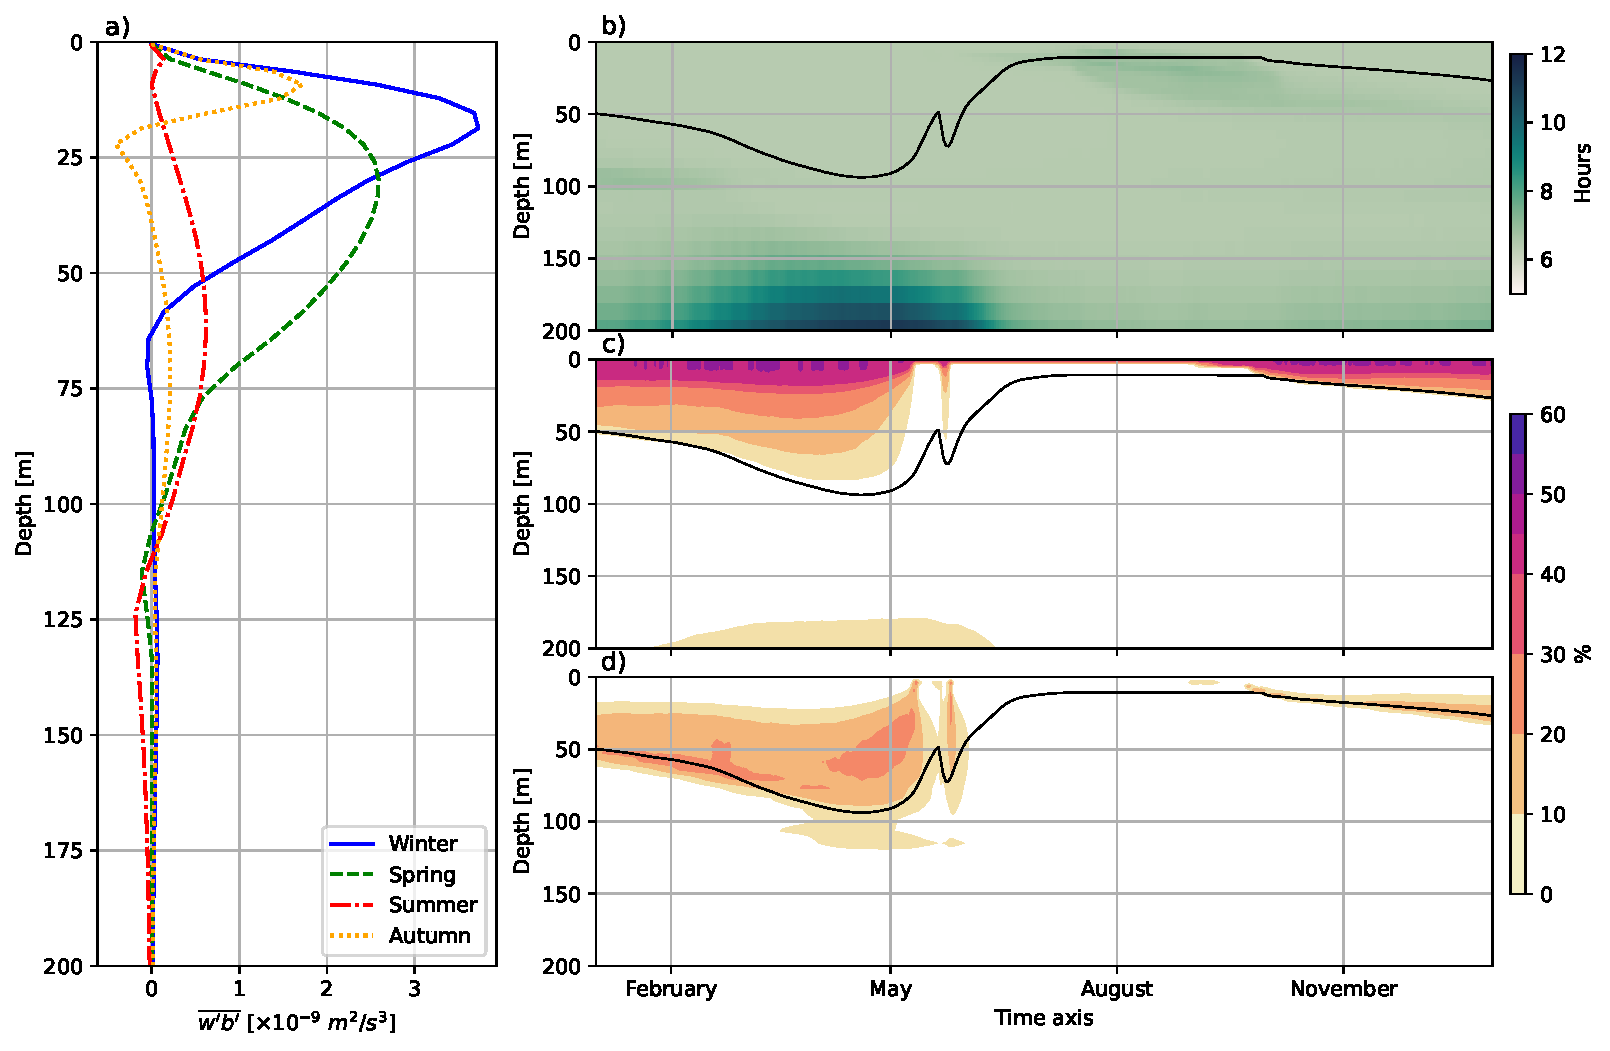
\includegraphics[width=1\textwidth]{Fig_8_WpBp_bRi_and_angle.pdf}
  \caption{a) Profiles of the spatially averaged energy conversion term from EPE to EKE ($w'b'$; Eq. \ref{eq:eq4}) for each season. Hovm\"oller diagrams of b) the Eady time-scale (Eq. \ref{eq:eq14}), c) the horizontal probability of the balanced Richardson angle to meet the ageostrophic instability criteria (Eq. \ref{eq:eq12}), and d) the horizontal probability of the balanced Richardson number to meet the baroclinic instability criteria ($Ri \sim O(1)$). The black solid lines in panels b, c, and d show the ML depth.}
  \label{fig:fig_8}
\end{figure}

The baroclinic energy conversion shows a winter enhancement of baroclinic instabilities and a decrease in summer. To better understand the seasonality of instabilities, we examine the Eady time scale, and the occurrence of ageostrophic and baroclinic instabilities. Longer Eady time scale are found in summer ($>8\ hrs$; Eq. \ref{eq:eq14}; Fig. \ref{fig:fig_8}b). In winter and spring, instabilities grow quicker, consistent with the development of submesoscale variability due to ML instabilities. Using a simple linear model, \citet{Ou_dissipation_1986} showed that friction beneath sea ice rapidly damps an eddy field within days, slower than the fastest-growing mode on the Eady timescale. This implies that dissipation acts slower than the growth of ML instability, thereby resulting in a weak but persisting submesoscale field under sea ice. Overall, the ageostrophic linear theory suggests a rapid growth of submesoscale motions in winter and a slower growth in summer \citep{FoxKemper_eddies_2008}.

% The horizontal probability of the occurrence of ageostrophic instability confirms that instabilities are present in the simulation.
In our simulations, values lower than the local criteria described in Eq. \ref{eq:eq12} and $Ri \sim O(1)$ correspond to the likely occurrence of various ML ageostrophic instabilities and baroclinic instabilities \citep{Thomas_symmetric_2013,Haine_instability_1998}. Figure \ref{fig:fig_8}c shows the percentage of horizontal grid cells in which the local criteria for ageostrophic instabilities is met. These instabilities occur in $\sim 50\%$ of the domain within the ML between November-June, because surface buoyancy forcing during ice formation drives convective instabilities. During the ice-free months, the stability of the water column increases, making ML ageostrophic instabilities less likely to occur near the surface. Figure \ref{fig:fig_8}d shows the percentage of horizontal grid cells in which the local criteria for baroclinic instabilities is reached. The likelihood of baroclinic instabilities to occur is located between the region with high probability of ageostrophic instabilities and the ML base, where the isopycnals are tilted. The maximum probability within the domain is reached during the melting period (April - June) with values of $\sim 30\%$. Regardless of the presence of baroclinic instabilities, ageostrophic instabilities are the main source of energy required for submesoscale to persist underneath the sea ice cover.

\begin{figure}[t!]
  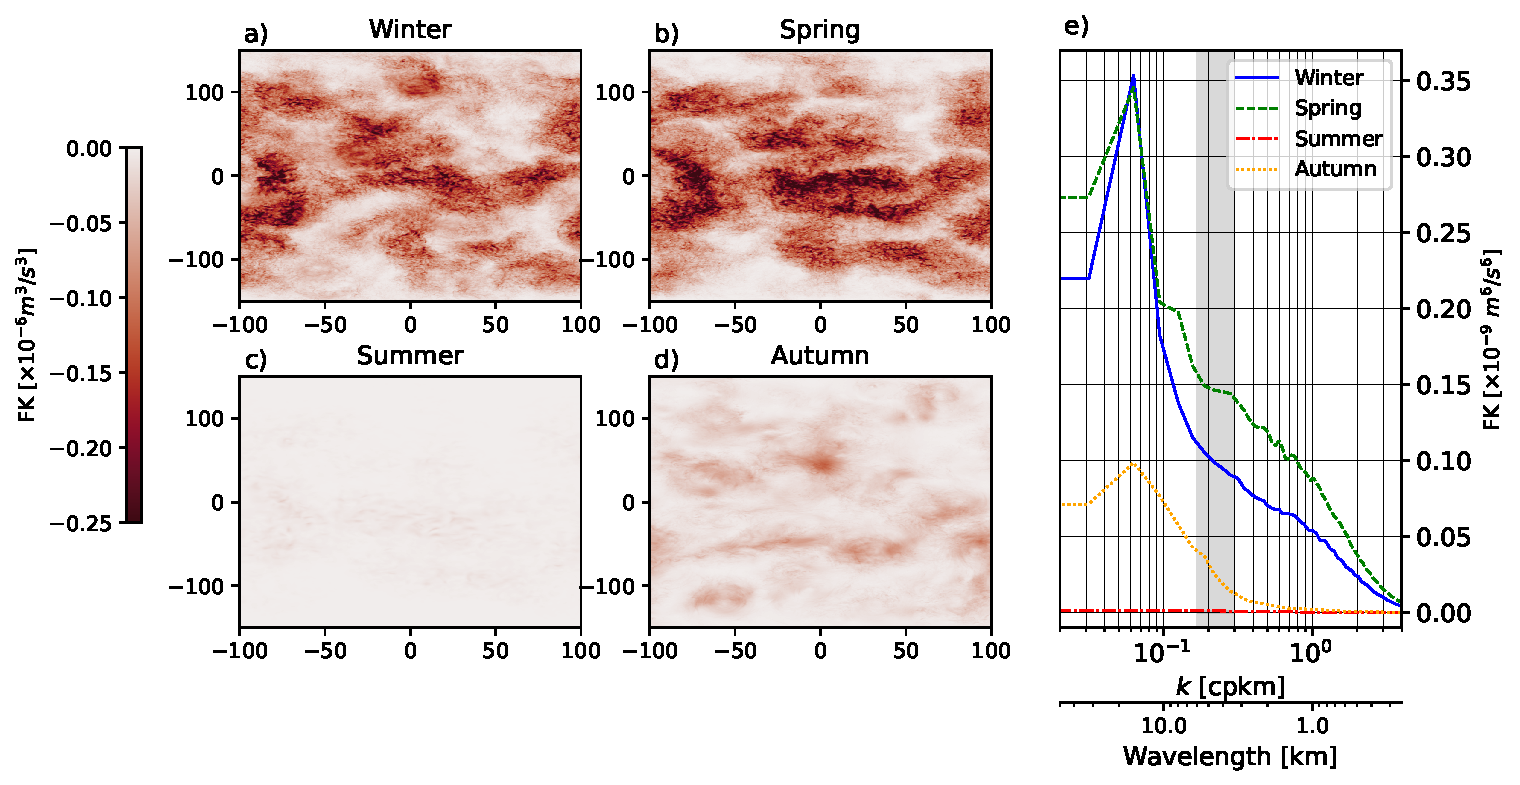
\includegraphics[width=1\textwidth]{Fig_9_eddy_killing.pdf}
  \caption{Spatial pattern of the mean ice-induced eddy dissipation term (or ice work) for a) winter, b) spring, c) summer, and d) autumn. e) Seasonal spectra of the ice-induced eddy dissipation term. The grey vertical shaded area in pannel e) correspond to the Rossby radius ($R_D$) range within the second year of the simulation.}
  \label{fig:fig_9}
\end{figure}

A sink of energy in the ML of our simulation is the dissipation due to the presence of sea ice. Figure \ref{fig:fig_9} shows the averaged seasonal ice-induced eddy dissipation term estimated from Eq. \ref{eq:eq18}. In winter and spring, the ice-covered seasons, the domain averaged ice-induced eddy dissipation is the largest at rates of $-6.8\times10^{-8}\ m^3/s^{3}$ and $-7.9 \times10^{-8}\ m^3/s^{3}$, respectively. As regions of the domain transition from ice-covered to ice-free and the ice concentration decreases from $\sim 100\%$ to $0\%$, the ice-induced eddy dissipation in ice covered regions becomes almost negligible at $-2.3\times10^{-9}\ m^3/s^{3}$, since the ocean velocities and ice velocities are similar (Fig. \ref{fig:fig_4}b). Once the ice starts to grow again in September, the magnitude of the ice-induced eddy dissipation increases to $-1.8\times10^{-8}\ m^3/s^{3}$. Furthermore, the spectral estimate of the ice-eddy dissipation shows the dominant scale in which the ice-induced eddy dissipation acts (Fig. \ref{fig:fig_9}e). The spectra peaks at scales of approximately $15\ km$, within the mesoscale range all year around, being the largest in winter and spring. At smaller scales than mesoscale, the spectra decrease in magnitude. Thus, the ice-induced eddy dissipation strongly dissipate mesoscale, while the submesoscale experiences a weaker ice-induced dissipation, consistent with the KE fluxes shown in Figure \ref{fig:fig_7}c.

\section{Discussion \& Conclusions}
\label{conclusions}

The pronounced seasonality of the mesoscale, submesoscale, and KE in seasonally ice-free oceans is largely driven by the interplay between eddies and sea ice. During summer, the absence of sea ice allows for the transfer of energy from smaller-scales (submesoscale) to larger scales (mesoscale) through an inverse energy cascade, resulting in the development and persistence of mesoscale eddies in summer. In winter, submesoscale is generated by ML instabilities and sea ice induces eddy dissipation (analogous to eddy-killing), preferentially dissipating the mesoscale range of motions. Note that when the ice is mobile (i.e. at low ice concentrations), the ocean and ice scales of motion become similar and thus the stress is negligible. Meanwhile, when the ice is compact (high ice concentration), the ocean and ice scales of motion are different, and thus the stresses are larger. Thus, the seasonality of the inverse energy cascade and ice stress leads to a more active mesoscale field in summer and a weaker one in winter, while the submesoscale field is stronger in winter and weaker in summer. Therefore, in the seasonally ice-covered regions, the dynamical interactions between the ice and ocean can modulate the seasonality of the eddies and KE. Yet, it remains to include the interactions with the atmosphere (i.e. including winds) that can modify the sources and sinks of energy of the sea ice and the ocean. 

Our results are consistent with previous studies suggesting that the regions of high ice concentration lack a seasonal cycle of the energy at mesoscale \citep{Mensa_seasonal_2017}, while regions with varying ice concentrations have a pronounced seasonality of the most energetic scales \citep{Manucharyan_eddies_2022, Liu_seasonal_2024}. This is likely consistent with observational evidence \citep{Cassianides_eddies_2023}, but more observational data is required to corroborate it. Notably, the seasonality of scales and KE under ice cover differs from the seasonality of ice-free oceans, where mesoscale contains most of the KE in summer, while in winter the KE slightly decreases in the mesoscale and increases in the submesoscale \citep{Callies_seasonality_2015}. Previous studies such as \citet{Manucharyan_eddies_2022} described qualitatively that the seasonality of eddies is controlled by dissipation in the presence of sea ice and a summer dominated by mesoscale-driven frontogenesis. Our work is complementary to this, since as previously hypothesized, the ice-induced dissipation is important on dissipating mesoscale in winter. Maybe more importantly, the KE flux analysis reveals that dissipation in conjunction with an inverse energy cascade are responsible for the seasonality of the mesoscale and submesoscale fields.

Our idealized setup builds intuition upon ignoring the effect of winds. Yet, the winds are likely crucial also in the seasonality of the KE in the Arctic Ocean, as it is generally considered the main input of energy to the ocean \citep{Ferrari_KE_2009}. Despite this, sea-ice can act as a barrier to the wind forcing, and thus the ocean scales of motion and KE may experience a different seasonality, particularly since the Arctic is characterized by strong winds and surface stress in winter and weaker winds and surface stress in summer \citep{Hughes_winds_2015, Martin_stress_2014}. In regions with thick, high concentration of sea-ice and slow moving sea ice in winter, the winds may have little to no impact in the ocean scales of motion, thus KE will retain a similar seasonality as discussed here and consistent with \citet{Manucharyan_eddies_2022}. However, in regions with highly mobile sea-ice in winter, the interplay of winds, sea-ice, and ocean is more complex, since the winds will control the scales and rates of ice and ocean motions and thus modulate the ice-induced eddy dissipation and energy across all oceanic scales of motion.

Finally, regions with thin and low concentrations of sea ice (i.e. in the Marginal Ice Zone) will likely be energized by the winds in winter and thus the seasonality of the scales and KE may resemble more that of the open ocean, in which both mesoscale and submesoscale are present in winter, but only mesoscale remains in summer \citep{Uchida_seasonal_2017}. 
Despite all this, the sea-ice ocean-atmosphere interactions are likely more complex and thus they should be explored further to better understand how wind forcing impacts the seasonality of scales and KE in the ocean at different ice concentrations and thicknesses. This is important since the coupling between the ocean, ice, and atmosphere will modulate both the seasonality of the ocean scales, sea-ice roughness, and the ice-induced eddy dissipation synchronously.
Additionally, changes in stratification, particularly the strength and depth of the halocline, are expected to modulate the dominant length scales of eddies. Stronger stratification (i.e., a shallower or sharper halocline) can limit vertical motions and reduce the eddy length scale, while weaker stratification can enable larger-scale features. However, we hypothesize that this will not significantly alter the overall seasonality: eddies will remain larger than the $R_D$ in summer and smaller than $R_D$ in winter, maintaining the same seasonal pattern although their length scales will readjust to stratification changes.


We use an elasto-visco-plastic rheology, but we hypothesize that using a different rheology or even a discrete floe-resolving sea ice models will qualitatively reproduce similar ocean scale seasonality. This is because the key processes, such as the seasonality of the inverse energy cascade and ice-induced eddy dissipation, are inherent to the coupled interactions between the ice and ocean. However, changes in the strength of the sea ice internal, collisional stresses and/or roughness may modulate the intensity of the ice-induced eddy dissipation and the temporal evolution of the ocean scales of motion. For example, a smaller roughness value will lead to a weaker stress and thus a weaker ice-induced eddy dissipation and a more energetic ocean. A different rheology will likely change the ice-roughness and thus also modulate the response of the ice-induced eddy dissipation.


The processes described here could have significant implications for the future of the Arctic Ocean. As the Arctic warms and sea ice continues to diminish, particularly during the summer, the Arctic eddy field is expected to become more energetic \citep{Kim_ice_free_2023, Li_eddy_2024}. As the Arctic transitions to an ice-free summer, the seasonality of the inverse energy cascade, along with changes in the buoyancy fluxes, will modulate the persistence and energetics of the mesoscale field during the summer months. Additionally, the winter sea ice concentration and thickness have also decreased over the last few decades and are expected to continue to decline in the future \citep{Wang_ice_trends_2019}, thus the ice-induced eddy dissipation may further weaken in the future, potentially altering the established seasonal energy cycle of the mesoscale and submesoscale in the Arctic. Therefore, understanding of the seasonality of the Arctic Ocean KE is crucial for predicting the Arctic Ocean's energy distribution and variability, and its evolution in response to the ongoing changing climate.

\section{Open Research}
The idealized model configuration of the model is described and publicly available via \url{https://doi.org/10.5281/zenodo.14204424} \citep{martinez_moreno_2024_config}.
All analyses and figures in this manuscript are reproducible via Jupyter notebooks and instructions can be found in the Zenodo archive \texttt{Ice-Ocean KE seasonality} via \url{https://doi.org/10.5281/zenodo.14204488} \citep{martinez_moreno_2024_repository}.

\section{Conflict of Interest Statement}
The authors have no conflicts of interest to disclose.

\acknowledgments
We thank the two anonymous reviewers, Dr. David Marshall, and the editor Dr. Stephen Griffies for their constructive comments and suggestions that helped to significantly improve the manuscript.
We acknowledge funding from the ANR ImMEDIAT project (ANR-18-CE01-0010) and the MEDLEY project funded by the program JPI Ocean/JPI Climate (ANR-19-JPOC-0001) project. The idealized simulations and their analysis were performed using the HPC facilities DATARMOR of ’Pôle de Calcul Intensif pour la Mer’ at Ifremer, Brest, France.

\bibliography{biblio}

\end{document}
